\chap{A Mobile Behaviour Change Intervention Framework} \label{chapter: prevention-framework}

\setlength{\epigraphwidth}{.50\textwidth}
\begin{epigraphs}
\qitem{Reducing risks to health is the responsibility of governments – but not only of governments. It rightly remains a vital preoccupation of all people, in all populations, and of all those who serve them.} %Quote
{--- \textsc{Dr. Gro Harlem Brundtland} \\ \textit{The World Health Report, 2002}}
\end{epigraphs}

This chapter details the design and development of a mobile behaviour change intervention framework for acute and chronic health conditions. The chapter begins by detailing what behaviour change interventions are, the existing behavioural models, and how technology may improve various aspects, including reporting, engagement and progression. From analysing the existing evidence, and various stakeholder's needs, a set of requirements and procedural steps are established to guide the development of a technological intervention.
The framework is then applied to the area of AD and an app aiming to reduce AD risk for it's users is developed.

\section{Introduction}
As mentioned in the previous chapter, Chapter \ref{chapter: lit-review}, AD has a number of modifiable risk factors which may be targeted through behaviour change. Many of these behaviours are not unique to AD risk, but are shared amongst many of the leading causes of mortality, including heart disease and stroke. As a result an effort to mitigate disease risk for one disease, may also significantly minimise risk of another. There is therefor great imperative for the creation of a behaviour change framework which can be adapted to any modifiable disease, and the opportunity to evaluate the approach in a relatively uncharted area, AD prevention. To create this technology framework however, one must explore the psychology of behaviour change and identify the opportunities for technology injection.

\section{Behaviour Change Interventions}
The altruistic goal of all public health interventions is to lower the incidence of poor health, disease and suffering. Many adverse health problems are caused directly by human behaviours, such as substance use, smoking, overeating, alcohol consumption and unprotected sexual intercourse. All of these behaviours are theoretically controllable, yet many exercise little or no-control over them. A key question for health behaviour research is how to modify the current behaviours which cause increased risk, and promote the adoption of healthier, less risky behaviours.
A number of strategies have been used by governments, health officials and researchers to reduce health risks. They can be broadly categorised as interventions that aim to reduce risk in the population as a whole, and those that target individuals within the population \cite{Guilbert2003}. The former include interventions by government, through legislation, tax and financial incentives; engineering solutions such as the provision of piped water; and health promotion campaigns targeting the general public \cite{Guilbert2003}. The latter includes interventions to change behaviours of individuals, typically at a personal level (e.g., personal interaction with their health provider or general practitioner).
Behaviour change programs are a relatively recently public health-related term, and have evolved over time since the 1980's when much of the scientific research began. Understanding of the specific processes involved in an individual's behaviour change has increased during this period and most behaviour change interventions now share the same basic characteristics and components.

\section{Existing Methods and Opportunities}
This section will examine the existing methods of delivering a behaviour change interventions, including modelling behaviours, reporting behaviours and analysisng behaviours.

\subsection{Modelling Behaviour Change}
There are a number of ways in which an individuals behaviour change can be theoretically modelled \cite{Morris2012a}. These include the widely cited and applied Theory of Planned Behaviour (TPB) \cite{Ajzen1985}, the Health Belief Model (HBM) \cite{Hochbaum1958, Sharma2012} and the Transtheortical Model (TTM) \cite{Prochaska2005, Prochaska2013}. The most apt models for planning a behaviour change intervention, however, are the HBM and the TTM. The TPB is useful in predicting certain behaviours, and for retrospective analysis, but is not considered useful or effective in relation to designing and planning an intervention that should result in behaviour change \cite{Hardeman2002}.

\subsubsection{Health Belief Model}
The HBM is a cognitive behaviour model that posits that a persons behaviours are determined by a belief or perception of threat to their health, and the outcomes of specific actions \cite{Morris2012a}. Additional stimulus can be added to these existing beliefs to trigger a want to change or an adoption of behaviour. Use of additional stimulus is referred to as a `\textit{cue to action}'. The use of fear or perceived threat is at the core of this model and also relies upon on the self-efficacy of the person to correct their own behaviours. \citeauthor{Nisbet2008}, \citeyear{Nisbet2008}, summarise the model in the following manner:
\begin{displayquote}
	``In order for behaviour to change, people must feel personally vulnerable to a health threat, view the possible consequences as severe, and see that taking action is likely to either prevent or reduce the risk at an acceptable cost with few barriers. In addition, a person must feel competent (have self-efficacy) to execute and maintain the new behaviour. Some trigger, either internal (e.g., bodily symptoms) or external (e.g., a public service ad), is required to ensure actual behaviour ensues'' \cite{Nisbet2008}.
\end{displayquote}

Fear appeals\footnote{the use of persuasive messages to stimulate fear based on harmful outcomes that are associated with certain lifestyle practices} have been used extensively for over 60 years in public health interventions \cite{Ruiter2014, Rice2012}. Perhaps not surprisingly, they have been found to be rather ineffective and can produce a polarising effect within the intended cohort \cite{Ruiter2014}. Since most people wish to think of themselves as healthy, such threatening information can lead to a defensive response, motivating intended recipients to avoid exposure to the material in the future \cite{Ruiter2014}. An example of a public health campaign aiming to use fear appeal can be observed globally in tobacco packaging via the use of clear warning messages and graphic images of smoking related diseases.

\subsubsection{Transtheoretical Model}
The TTM is a stage theory that is often used as a guiding framework for many health-related interventions. This model posits that an individual’s willingness to make behavioural changes is driven by their readiness to change. The stages of readiness are described as pre-contemplation, contemplation, preparation, action and maintenance, with relapse to prior unhealthy behaviours possible between the action and maintenance stages \cite{Prochaska2005}. The traversal of these stages can be seen in Figure \ref{fig: ttm-model}.

\begin{figure}[h]
    \centering
    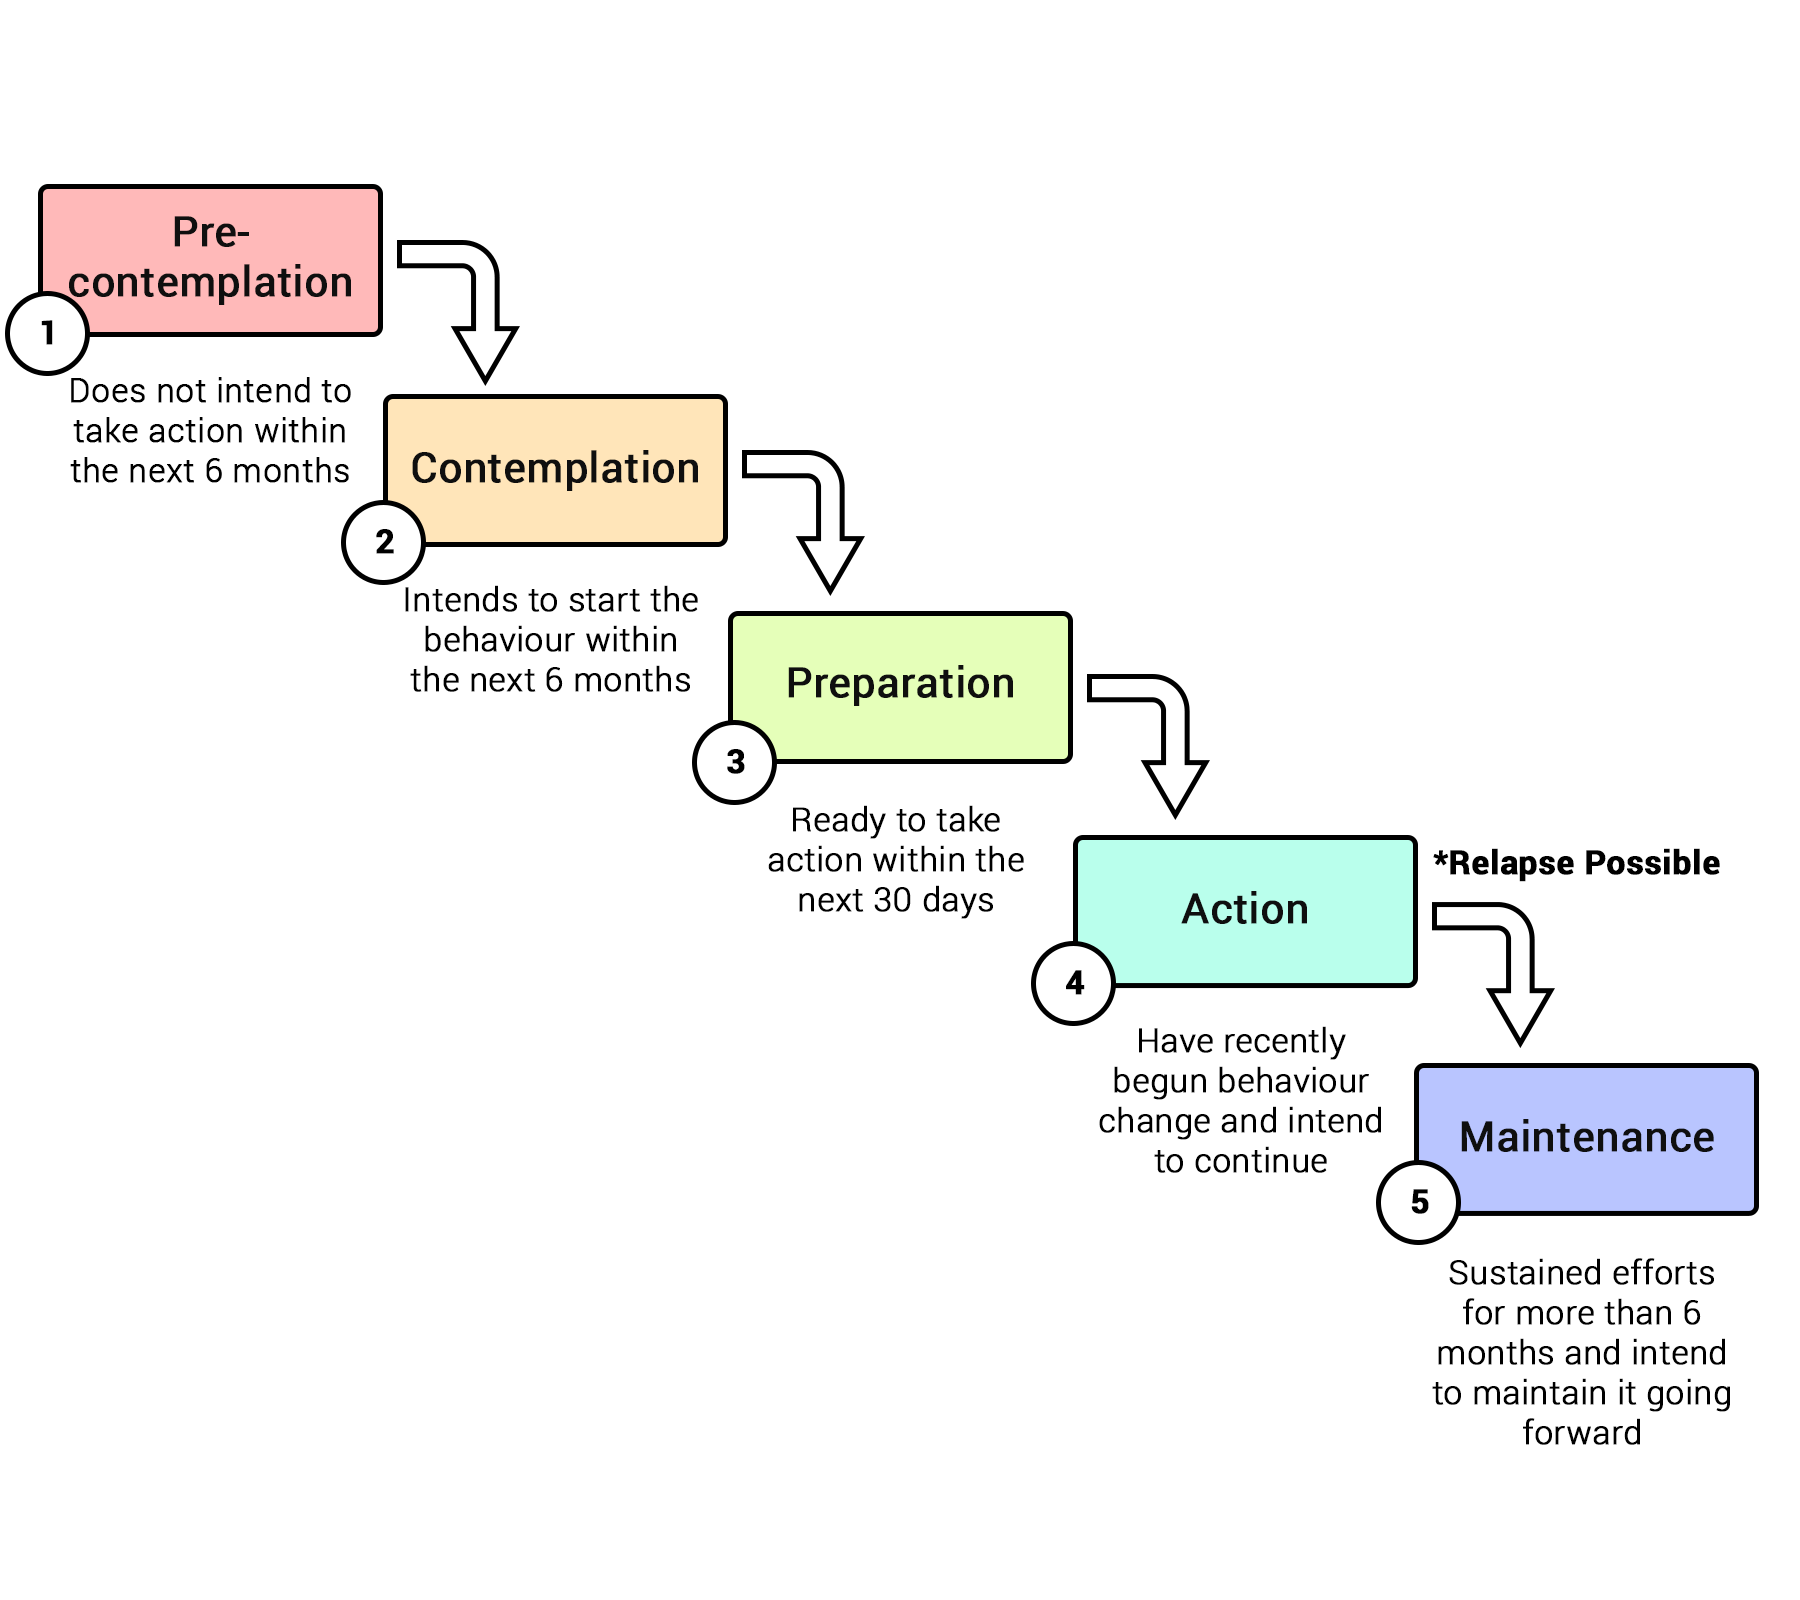
\includegraphics[scale=0.16, angle=0]{Files/prevention-study-1/figures/ttm-stages-model}
    \caption{Stages of behaviour change within the transtheoretical model}
    \label{fig: ttm-model}
\end{figure}


The model was first developed in relation to smoking cessation, but has since been adapted and applied to various other behaviours \cite{Nisbet2008}. The benefit of the stage model is that individuals who are at the same stage will be facing similar challenges, and therefor can be aided with the same style of intervention \cite{Morris2012a}. Each stage consists of various processes, seen in Table \ref{tbl: ttm-states-description}, which are carried out by the individual before they progress to the next stage.

\begin{sidewaystable}[ph!]
\centering
\caption{Stages and Processes of the Transtheoretical Model of Behaviour Change}
\label{tbl: ttm-states-description}
\resizebox{23cm}{!}{% Resize
\begin{tabular}{llll}
\hline
Stage & Stage Definition & Process & Process Definition \\ \hline
\multirow{3}{*}{Pre-contemplation} & \multirow{3}{*}{\begin{tabular}[c]{@{}l@{}}Individual is unaware of the problem; \\ No intention to change in foreseeable future\end{tabular}} & Consciousness raising & \begin{tabular}[c]{@{}l@{}}Increasing information about \\ self and problem\end{tabular} \\
 &  & Dramatic relief & \begin{tabular}[c]{@{}l@{}}Experiencing and expressing feelings \\ about problems and situation\end{tabular} \\
 &  & Environmental re-evaluation & \begin{tabular}[c]{@{}l@{}}Assessing how one's problem \\ affects physical environment\end{tabular} \\ \hline
Contemplation & \begin{tabular}[c]{@{}l@{}}Individual is aware of the problem; \\ Serious consideration of change in behaviour\end{tabular} & Self-re-evaluation & \begin{tabular}[c]{@{}l@{}}Assessing how one feels and\\ thinks about oneself with \\ respect to a problem\end{tabular} \\ \hline
Preparation & Individual is intending to take action & Self-liberation & \begin{tabular}[c]{@{}l@{}}Choosing and commitment \\ to act or a belief in ability to change\end{tabular} \\ \hline
\multirow{4}{*}{Action} & \multirow{4}{*}{\begin{tabular}[c]{@{}l@{}}Individuals modify their behaviours, experiences \\ and/or environment in order to overcome problem\end{tabular}} & Counter-conditioning & \begin{tabular}[c]{@{}l@{}}Substituting alternatives for problem \\ behaviours\end{tabular} \\
 &  & Stimulus control & \begin{tabular}[c]{@{}l@{}}Avoiding or countering stimuli that \\ elicit problem behaviours\end{tabular} \\
 &  & Helping relationships & \begin{tabular}[c]{@{}l@{}}Being open and trusting with \\ problems to someone\end{tabular} \\
 &  & Reinforcement management & \begin{tabular}[c]{@{}l@{}}Rewarding one's self or being \\ rewarded by others\end{tabular} \\ \hline
Maintenance & Individual works to prevent relapse and consolidate gains & Social Liberation & \begin{tabular}[c]{@{}l@{}}Increasing alternatives for \\ non-problem behaviours available \\ in society\end{tabular} \\ \hline
Relapse & Individual's behaviours relapse to any previous stage & Re-engagement & \begin{tabular}[c]{@{}l@{}}Reminding one's self of previous\\  effort to change behaviour\end{tabular} \\ \hline
\end{tabular}
}
\end{sidewaystable}

\subsection{Aiding Progression via Technology Injection}
From the literature review it was identified that there are various opportunities for technology to support the necessary processes at each stage in the TTM (See Table \ref{tbl: ttm-states-description}, especially within the contemplation, preparation and action stages.

\subsubsection{Contemplation}
The contemplation state posits that the individual is aware of the problem and is serious in their consideration of changing their behaviour. The process associated with this state is \textit{Self-Re-evaluation}, which is an assessment of how one feels and thinks about oneself, with respect to the problem. The key to his process for the individual is understanding the problem and understanding their behaviour. This can be facilitated through technology by education of risk factors, presentation of current behaviours effect on risk and suggesting tools for support.

\subsubsection{Preparation}
The preparation state posits that the individual is intending to take action, typically within the next 30 days. The process associated with this state is \textit{Self-liberation}, which is when the individual commits to act or truly believes in their ability to change. At this point, technology can benefit the individual through ease of accessibility, both software and hardware based. This is especially the case for smartphone apps.

\subsubsection{Action} \label{subsubsection: ttm-action-phase}
The action state posits that the individual is now actively changing their behaviours, their experiences or the environment in order to address the problem. The action state contains numerous processes, each with their own opportunities for technology injection.

\textbf{Reinforcement management.} This process rewards the individual for their efforts and achievements, either by one's self or by others. Technology has numerous ways by which to deliver rewards, from other individuals, or from the technology itself. In the case of smartphone apps, rewards may be given as digital trophies and achievements, or by unlocking further content-material. Such techniques are referred to as gamification, and their use has been explored in recent behaviour change studies \cite{Schoech2013}.
\newline \textbf{Helping relationships.} This process requires the individual to be open and trusting with problems to someone else. Technology can aid this process by providing access to controllable social support networks, in which support and praise can be given. These social networks would allow individuals to share their current progress, achieved milestones and provide \& receive support from others at the same stages in their behaviour change. The use of social networks in promoting healthy behaviours has shown numerous benefits, including acting as a motivator to exercise and expanding food choices \cite{Vaterlaus2015, Kamal2014}.
\newline \textbf{Counter-conditioning.} This process involves substituting alternatives for problem behaviours (e.g., Replacing high-sugar drinks with fresh fruit drinks). Technology can help educate the individual on suitable alternatives at the point of need through information access \cite{Kamal2014, Hermawati2014, Dunford2014}. Such work has been performed with those whom diet choices can have an acute effect (e.g., diabetics) \cite{Klonoff2013}, but has not been extended for improving behavioural choices within currently healthy individuals, with the aim of observing long-term health benefits.
\newline \textbf{Stimulus control.} This process involves avoiding or countering stimuli that can elicit problem behaviours. Technology's opportunities here are somewhat limited. Ubiquitous computing researchers have envisioned scenarios in which ``just-in-time'' technologies, harnessing information about location, past-activities and user-context, can detect when a user would require assistance to motivate them to avoid negative outcomes \cite{Intille2004}. An example use-case would be the detection of fast-food outlets in the user's proximate location and the current time is lunch time, thus inferring the user is going to eat fast food. The user would then receive an alert or some form of contact from the technology advising them to avoid this action.

\subsection{Reporting Behaviours} \label{subsection-reportingbehaviours}
To accurately assess the effect of a behaviour change intervention, the validity of the behaviours reported must be accurate. There are numerous methods by which behaviours can be recorded within an intervention, including diaries, self-reporting questionnaires, direct observation and by proxy reports \cite{Elliott2014}.

\subsubsection{Diaries}
Diaries present a low cost, easily maintained and time efficient method of recording behaviours, however, are open to cognitive bias due to subjective self-assessment and rely heavily on the person’s ability to accurately recall past events \cite{Stone2002}.

\subsubsection{Direct Observation}
Direct observation offers health investigators an accurate portrayal of behaviours within the given window of observation \cite{Prince2008}. They are believed to offer more truthful recordings and can be used as a method to increase precision and accuracy for the purposes of validating self-reported behaviours. With regard to monitoring physical behaviours, total energy expenditure can be calculated using calorimetry (i.e. double labelled water), heart rate monitors and motion sensors \cite{Prince2008}. Whilst such approaches offer exceptional accuracy, they are intrusive, expensive and time intensive. It is also the case that the Hawthorne effect, commonly referred to as the observer effect, may change how an individual behaves under direct observation, and observations made may not be a true reflection of their behaviours outside of the observation window \cite{McCarney2007}.

\subsubsection{Self-reporting}
Self-reported questionnaires are commonly used in large-scale longitudinal studies, due to their uniformity in questioning, repeatability and ability to extract qualitative and quantitative information \cite{DiMarco2014}. Quantitative orientated questionnaires, seeking to gather quantifiable information about past-events, such as the ‘number of glasses of water consumed today’, can be at risk of cognitive bias and recall inaccuracy. Nevertheless, a comparative study seeking to validate previous day recall accuracy for active and sedentary behaviours when compared to direct observation found agreement of 85\% or higher in certain conditions, and suggests adults can accurately report their behaviours using previous day recall \cite{KozeyKeadle2014}.

\subsubsection{By proxy}
Proxy reporting is typically used when the subject in examination is somehow dependant on another adult, such as young children and the elderly. A study assessing the level of agreement between 6,425 children and their parents regarding dietary, physical and sedentary behaviours reported a mean agreement rate of 43\% \cite{Rebholz2014}. Similarly, studies assessing memory recall for the same events in children, young adults and the elderly showed that the reports of the elderly were as complete as the children’s, but were the least accurate overall \cite{Gawrylowicz2014}. This highlights both the potential inaccuracies of self-reporting within certain cohorts, and the need for ground-truth data due to the rate of disagreement found in reporting utilising a proxy.

\subsection{Improving Reporting via Ubiquitous Computing}
Whilst a variety of approaches can be employed to record behaviours, each has their own distinctive weaknesses relating to accuracy, repeatability, scalability and cost \cite{Prince2008}. The need for an objective mediator to draw agreement across the various approaches is desired. Pervasive computing may provide such a solution.

The widespread public adoption of smartphones, smartwatches, and wearable technology, has enabled computing to become truly ubiquitous. Wireless digital devices can enable the digitisation of individuals’ behaviours, often without the need for interaction. Wearable wrist-worn devices can be used to calculate an individual’s energy expenditure and step count \cite{Pande2013}, their current activity \cite{Cleland2013}, sleep quality \cite{Noor2013}, and heart rate \cite{Parak2014}. Smartphones, via the use of on-board accelerometers and GPS, can also track physical activity levels \cite{Ozdalga2012} and sleep efforts \cite{Min2014}, whilst various apps encourage self-reporting of food consumption \cite{Ozdalga2012}, enabling immediate calculation of calorie consumption. In addition, social media websites contain a plethora of social interactions that can be analysed for behavioural trends \cite{Ruths2014}. There is an abundance of potential use-cases for such technology in the self-management of one’s health, yet the adoption of this technology for the purpose of public health education or behavioural change interventions are extremely limited. Eric Topol, a physician who has been heavily involved with wireless medicine since its inception, states in his book:
\begin{displayquote}
``Our health care approach is reactive, and, as a result, we have a world of chronic diseases, most of which are poorly managed, such as congestive heart failure, high blood pressure, and diabetes, or not managed at all, as in the case of Alzheimer’s''
\begin{center}
	\rule{1cm}{0.4pt}
\end{center}
``Now comes a new wave of technology to not only improve the outlook for the chronic diseases of today but shift the capability, for the first time, to true prevention.'' \cite{Topol2012}.
\end{displayquote}

To leverage this opportunity, we must understand how to engage users with the new technology, and motivate them to ensure continual progression over time. Therefore, it is of paramount importance that maintaining engagement is highlighted as a key area of focus.

\subsection{Maintaining Engagement}
Evidence from internet based interventions suggest that repeated visits are necessary to achieve sustainable change \cite{Brouwer2011a}. Nevertheless, visitor engagement with these interventions is typically lower than expected, with many users opting out before becoming fully exposed to all the intervention material, resulting in suboptimal outcomes \cite{Brouwer2011a}. There is therefore the need to encourage and maintain engagement with interventions, whilst enhancing an individual’s motivations to return at a later date.

\subsection{Promoting Engagement via Technology}
Gamification is the application of game design techniques and mechanics to non-gaming domains \cite{Deterding2011}. To encourage engagement within a game, game designers utilise mechanics such as points, level-systems, avatars, badges, and leaderboards. These reward systems encourage continual progression, with the ultimate aim of maintaining engagement. Recently, there has been a surge of interest in the use of gamification for behaviour change studies, given that these reward systems help to promote engagement. Young adults and children are especially attracted to games, with virtually all young children having access to gaming consoles, computers and smartphone games \cite{Schoech2013}. As such, gamification elements have been used to educate and encourage desirable behaviours in children, such as increasing intake of fruits and vegetables through the use of fictional avatars \cite{Jones2014}, preventative education on substance-abuse and risk using smartphone and tablet apps \cite{Fiellin2014}, and an obesity prevention intervention via mobile and web platforms \cite{Delisle2015}. The use of gamification in adult behaviour change studies, however, is limited.
For health-conscious adults, commercially available smartphone apps and activity tracker companies, such as Strava, FitBit, and Nike, use gamification elements extensively in their efforts to maintain and promote continual engagement. Whilst each platform has their own approach they all record health related data, examples include monitoring physical activity levels, tracking meals and monitoring sleep quality. From these data various performance metrics are calculated from which achievements are rewarded, such as badges and trophies. In addition, a user can view, typically at a high level via interactive graphs, their performances across time, allowing them to become informed of their behaviours and their resulting outcomes. Social sharing of recorded data also plays a role in enabling gamification elements, such as leaderboards, allowing users to compare their efforts with those of others. Apple and Google, whose smartphone platforms combined, account for 96.3\% of the worldwide market share \cite{InternationalDataCorporation2015}, are now shipped with iOS Health kit and Google Fit services pre-installed. The aforementioned services are proprietary to their platforms, however, act to consolidate the available data of various health-related apps and activity trackers into one common interface. The inclusion of such services into the base functionality of the most extensively adopted smartphone platforms in the world, show the market’s anticipation of widespread adoption of health-related apps.
It is therefore hypothesised that the combination of constantly accessible, highly interactive, and individually tailored feedback, combined with gamification elements, such as rewards and leaderboards, would have the largest opportunity to maintain and encourage engagement with adults in a behaviour change study \cite{Middelweerd2014}, given the advantages that each elements brings.

\section{Stakeholders and Requirements}
%fix this up
This section details the development of a framework to guide the implementation of a technologically based approach to behaviour change interventions.

\subsection{The Stakeholders}
The stakeholders of any intervention consist of the End-User/Study Participant (EU), and the Health Investigator/Study-coordinator (HI)
The primary objective of the HI is to obtain accurate information on behaviours of the EU	, and their effects on observable health outcomes. The HI play a large role in the design of the intervention through the scope of their research question. As such, they majorly influence the non-functional requirements of a suitable intervention platform.

\subsection{Non-Functional Requirements}
From analysis of existing approaches of behaviour change interventions \cite{Prochaska2005,Ruiter2014}, commercial health promotion apps \cite{Ozdalga2012, Higgins2016} and software engineering best practices \cite{Fielding2000, Jones2010}, a number of non-functional requirements have been developed. These requirements are not specific `features' of a system, but rather are desired characteristics that influence the design of the system architecture.

\textbf{Accessibility.}
There should be minimal barriers/restrictions for the user to obtain the solution.

\textbf{Availability.}
The intended solution must be available to the user at the point of need.
\\The ability for HI to access or query user data must be as close to real-time as possible.

\textbf{Extensibility.}
The solution should facilitate data exchange between other health related apps to reduce the burden of duplicating user effort to enter data.

\textbf{Privacy.}
The solution must disclose to the user where their data is stored, who can access the data and permit the user to revoke access to their data.

\textbf{Security.}
Access control must be included for all users of the solution.
\\End-Users must register to use the solution and obtain content.
\\A single user may not view another users data.
\\Access to user data must require approved authentication from administrator.

\textbf{Scalability.}
Must be able to be used by varying numbers of users, and handle varying amounts of data.

\textbf{Tracking User Interaction.}
The solution must be capable of tracking user interactions with the system (e.g., tracking number of times a function has been used).

\textbf{Updatability.}
All content within the solution must be manageable by an administrator. This is important to keep content up-to-date as new scientific evidence becomes available.

\textbf{Usability.}
The solution must adhere to the selected platforms standards and follow best practice guidelines. This will reduce effort required to learn the solution and benefit the user through familiarity.

\textbf{Validity.}
All reported user data must be valid and testable. This includes dates, self-reported behaviours and interaction data.

\subsubsection{Platform Selection}
Consideration of the identified non-functional requirements narrows the scope of suitable platforms from which a solution can be developed. A number of key requirements directly influence the technology platform choice: Availability, Accessibility and Scalability.
Evidently, internet technologies and smartphones can address these  requirements, as they are now considered ubiquitous. As of March 2015, the smartphone surpassed the desktop in the U.S as the primary method to access the internet \cite{ComScore} (See Figure \ref{fig: graph-internetuse}).

\begin{figure}[h]
	\begin{tikzpicture}
	\begin{axis}[
		height=6cm,
		width=0.9\linewidth,
		%xlabel={Month},
		ylabel={\% Users},
		symbolic x coords={Mar14,Apr14,May14,Jun14,Jul14,Aug14,Sep14,Oct14,Nov14,Dec14,Jan15,Feb15,Mar15}
		]
	\addplot table [x=month, y=mobile, col sep=comma]{Files/prevention-study-1/data/internetuse.csv};\addlegendentry{Smartphone}
	\addplot table [x=month, y=desktop, col sep=comma]{Files/prevention-study-1/data/internetuse.csv};\addlegendentry{Desktop}
	\end{axis}
	\end{tikzpicture}
	\caption{Single Platform Users Share of Total Digital Population}
    \label{fig: graph-internetuse}
\end{figure}

This puts the smartphone in a unparalleled position as a suitable platform to deliver a health intervention to users. As such. for the general user, the smartphone should always be considered as the primary technology platform from which to base technological development.
There are some exceptions to this approach however, as in some cases additional analysis of technology ownership and literacy amongst the target cohort may need to be considered. For example, a technology-based intervention for seniors may require additional requirements gathering regarding the most suitable platform, given the negative correlation between age, smartphone ownership, and computing literacy \cite{Migo2015}.

\section{A Process Framework}
This section details the recommended procedure which should be followed to implement a technology based solution for health behaviour interventions.

\subsection{Examining Relationships}
Conceptually, the entities within the framework can be modelled in an entity relationship (ER) diagram, as seen in Figure \ref{fig: erd-model}.

\begin{figure}[h]
    \centering
    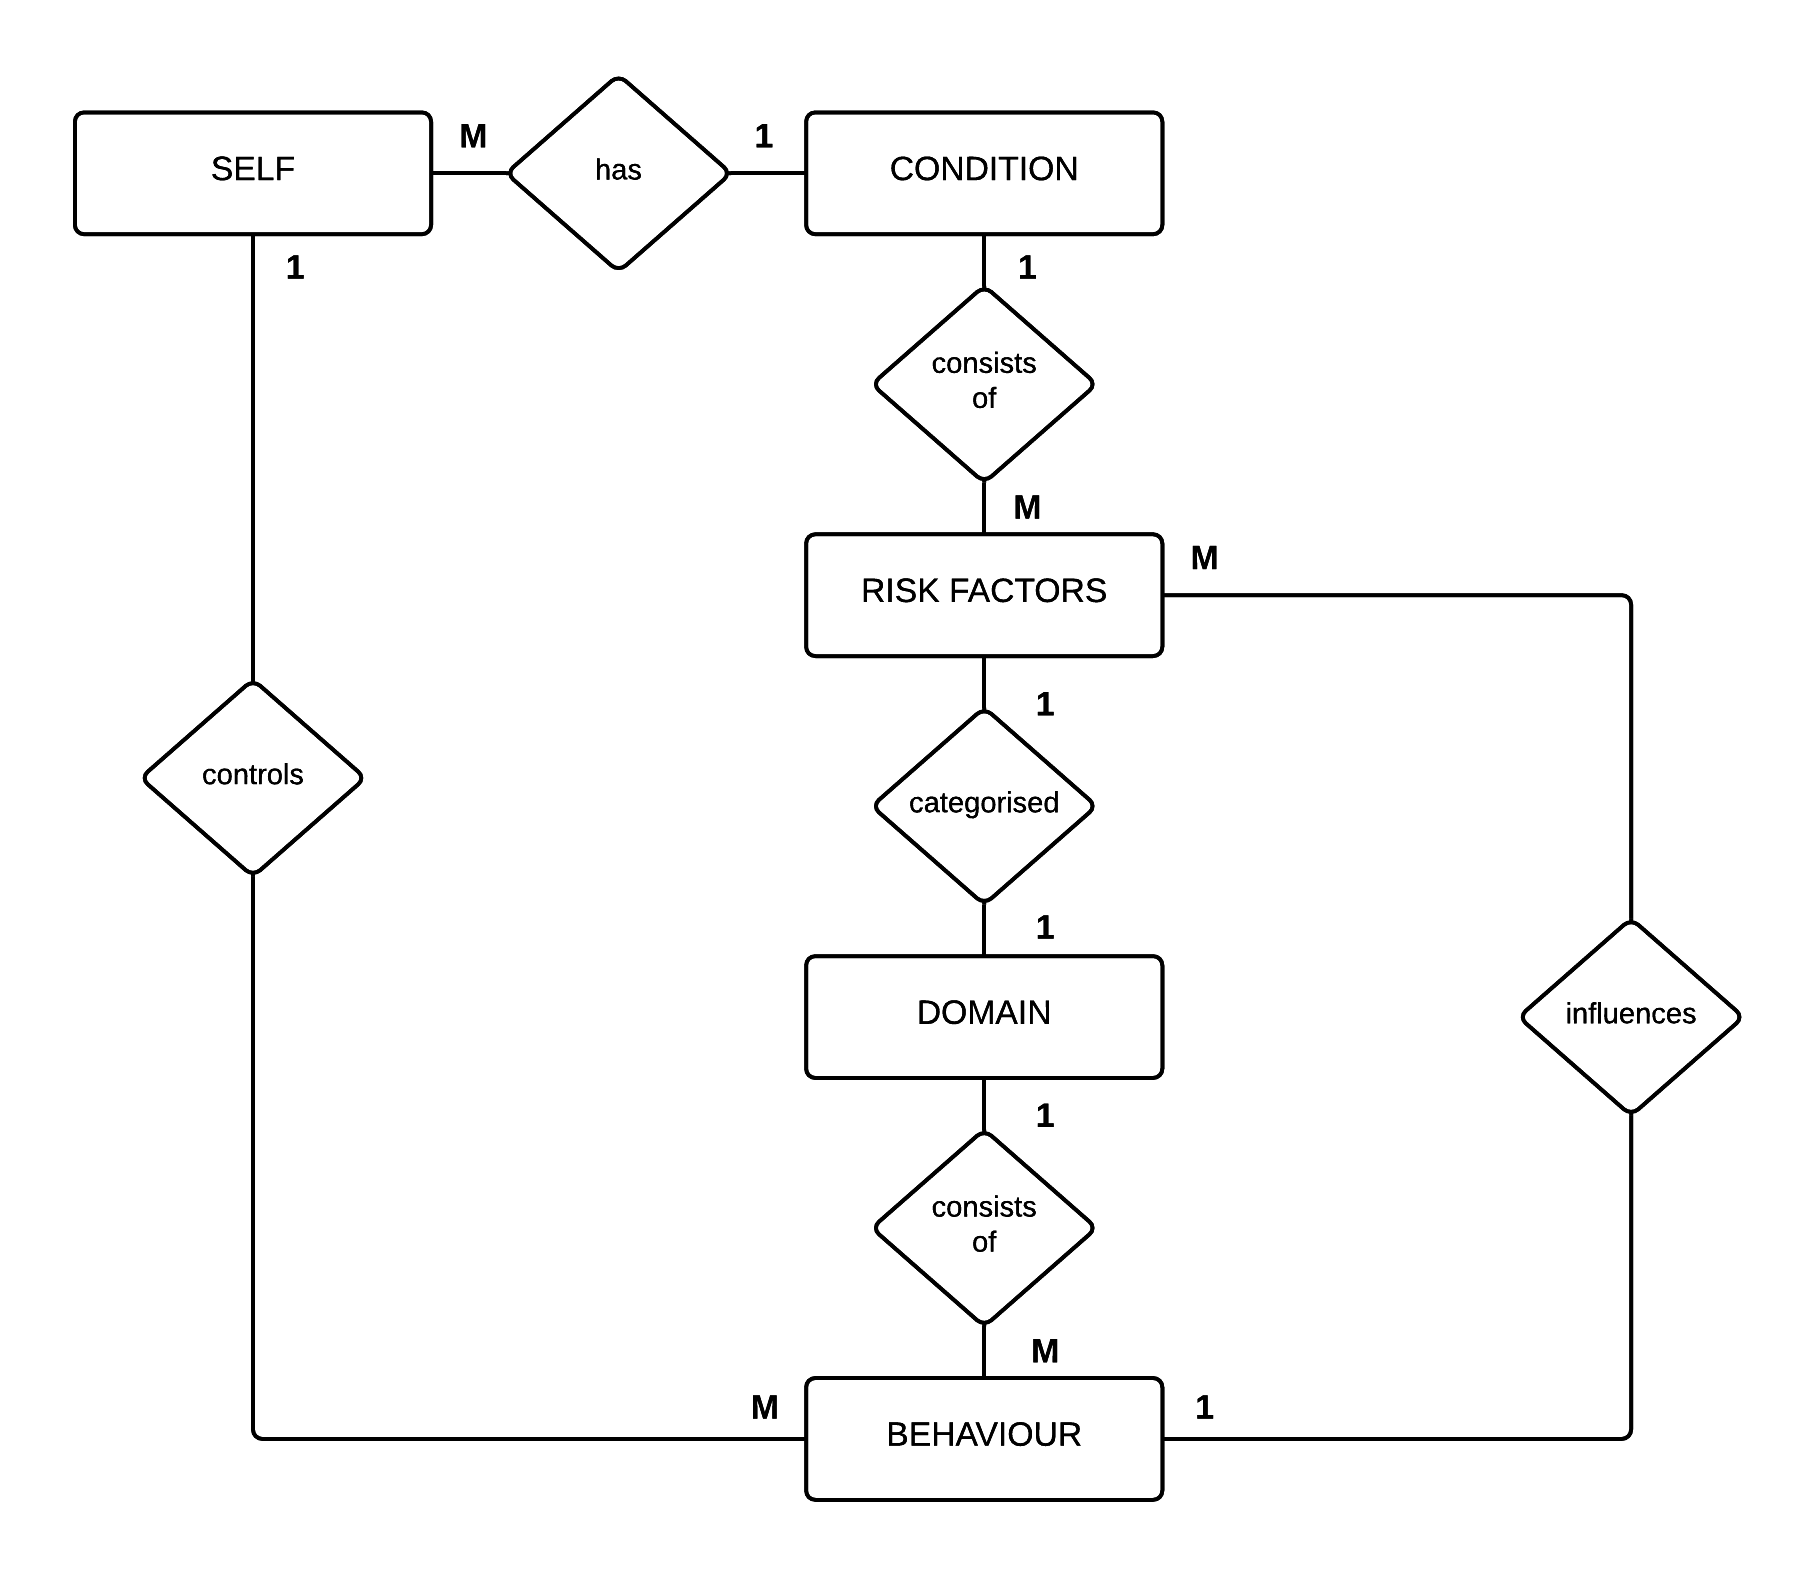
\includegraphics[scale=0.9, angle=0]{Files/prevention-study-1/figures/erd-riskfactors}
    \caption{Entity Relationship Model of Health Condition, Associated Risk Factors and Behaviours}
    \label{fig: erd-model}
\end{figure}

The ER diagram explores the interdependencies between a person (Self), their health condition, and its' associated risk factors, and behaviours. The model posits that a condition (e.g., Heart disease) consists of multiple risk factors (e.g., hypertension, obesity), which can be categorised into various high-level domains (e.g., stress, diet). These domains have associated behaviours (e.g., working long hours, high sugar consumption), which a person has direct control over. This control can be applied to influence the numerous risk factors and ultimately alter the status of the condition, both reactively and preventatively.

To create an health intervention program using the model described, each element must be understood in detail. The key is finding the shared information within each element, and this can be performed by following a logical ordered process.

\subsection{A Process Guide} \label{subsection: framework-process}
To guide the development of the technological intervention in the most effective manner, a procedural guide has been designed by the author. The guide details a strategy for each step of the process, based upon existing evidence and the available technologies.

The steps of the process are:
\begin{enumerate}[noitemsep,topsep=0pt]
\item Establish Condition of Interest
\item Establish Modifiable Behaviours
\item Establish Key Measures
\item Create Behavioural Targets
\item Generate Health Education Literature
\item Develop Education Delivery Mechanism
\item Develop Tracking Tools
\item Create Tools for Health Investigators
\item Evaluate via Expert Assessment
\end{enumerate}

\subsubsection{Clinically Focused}
The first 5 steps of the process are clinically focused and should be performed sequentially.

\textbf{1. Establish Condition of Interest} \\
The health condition which the intervention is to be targeted must be identified. A full literature review should be performed on the condition to establish the identified etiologies and risk factors.

\textbf{2. Establish Modifiable Behaviours} \\
Once all risk factors are established, each should be examined to establish those which are non-genetic, or modifiable. Modifiable risk factors are not limited to human behaviour, but also of the environment. Various environmental factors can be altered through behaviour change, and so should be considered \cite{Kujala2002}.

\textbf{3. Establish Key Measures}\\
For each modifiable risk factor, establish the standard methods of assessment. The format of these measurements are expected to be vary but by default will include physiological and behavioural measures.
\begin{itemize}[noitemsep,topsep=0pt]
\item \emph{Physiological} measures include quantitative measurement of the human structure, anthropometric assessments, uranalysis, and blood specimen analysis \cite{Oberg2014}.
\item \emph{Behavioural} measures include an array of behavioural assessments; including readiness-for-change, sleep quality, social engagement, depression, and couple satisfaction questionnaires  \cite{Martin2007}.
\end{itemize}

Additional measurements can be included on a case-by-case basis, depending upon the condition. For example, an intervention for a respiratory conditions may wish to use lung function tests, such as spirometry, whilst a focus on cognitive impairment may wish to use a battery of neurological examinations and brain imaging.

\textbf{4. Create Behavioural Targets} \\
Using the information established in steps 2 and 3, it is possible to set targets for desirable behaviours to mitigate the risk factors. Behavioural goals based upon scientific evidence may already exist, established by governments or health officials. Firstly, examine these existing recommendations. If more than one recommendation exists, use that which has the greatest scientific grounding for the targeted condition or age-group \cite{Stover2002, Pronk2004}.

\textbf{5. Generate Health Education Literature} \\
It may be necessary to repurpose the scientific literature identified in the previous steps into layman's terms\footnote{Using words and terms that the average individual, or someone without professional training in the subject area, can understand.}, depending upon its complexity.
There are a few general principles about education \cite{Gilbert2010} that should be considered:
\begin{itemize}[noitemsep,topsep=0pt]
\item To facilitate learning, repetition is generally required.
\item Recent experiences are more vivid than past.
\item Behaviours or skills must be practiced.
\item Learning is more effective when the learner is motivated by results.
\item The higher the education level, the greater the effectiveness of written word.
\item The lower the education level, the greater the need for visual or oral media.
\end{itemize}

Considering these principles, it is advised that a fact bank is created, containing short and impactful facts about the health condition. To supplement each fact, an example of a related behaviour and a positive health outcome should be attached. These should be presented to the user as often as possible to increase exposure and support learning. An example:
\begin{displayquote}
``Diabetes is the leading cause of blindness in working-age adults''
\begin{center}
	\rule{1cm}{0.4pt}
\end{center}
``Exercise is one of the most important things you can do to take control over diabetes. The key is to find something you enjoy doing and stick with it. It can be walking, swimming, cycling, or dancing — just get moving!. Aim for 30 minutes of activity, five days per week.''
\end{displayquote}

This format follows the principles of education, and presents a fact about the condition which motivates the person to act based upon desirable results. This is then reinforced through suggestions of actions to achieve the desired result. This particular example may be accompanied with visual cues related to blindness and exercise.

\subsubsection{Software Focused}
The latter stages are predominately software focused, but rely heavily upon on the quality and validity of the findings in the clinical stages. These stages can be performed concurrently and should be approached following an agile methodology.

\textbf{5. Develop Education Delivery Mechanism}\\
Using the health education literature, a suitable mechanism should be developed to present this information to the user. A mechanism unique to smartphones, and smartwatches, are notifications. These can be configured to be delivered at set times, or at particular contexts, inferred from sensors. Their representation may include badges, sounds or a custom text alert, as seen in Figure \ref{fig: notification-android}.
\begin{figure}[h]
    \centering
    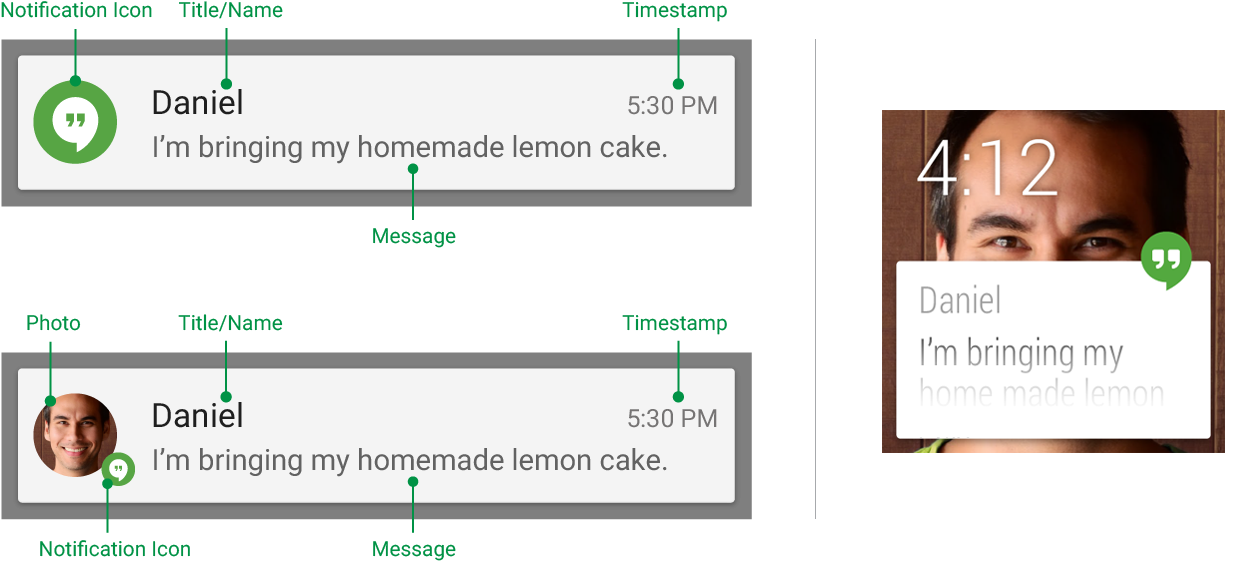
\includegraphics[scale=0.7, angle=0]{Files/prevention-study-1/figures/notification_android}
    \caption{Notification base structure for Android operating systems}
        \medskip
	\small
	Source: Image adapted from Android Developer Guidelines: Anatomy of a Notification \cite{NotificationsAndroid}.
    \label{fig: notification-android}
\end{figure}
The use of sound in notifications in smartphones is recommended to prompt the user to act upon them \cite{AppleNotifications2015} even if the user is not using the device. For the purpose of delivering the health education information in a notification, the amount of text should be limited. Having considered the principles outlined in Step 5, the fact portion is an ideal amount of text to display in the message body. Upon interaction with this text, the user may be presented with the additional lifestyle suggestion.

\textbf{6. Develop Tracking Tools} \\
To aid the progression of behaviour change, tools should be developed which allow the study participant to quantify their behaviours in the relevant domains. The tools may be a user interface, that allow for manual self-reporting of behaviours, or they may use existing data sources to extract relevant behaviours.

\textit{Goal Setting.} Primarily, the tools should encourage users to achieve the recommended targets identified in Step 4. These targets can be considered global targets, however, many individuals may require a tailored step-wise progression to reach these targets \cite{Prochaska2013}. Often when faced with targets that are deemed as unattainable, or too difficult, relapse occurs \cite{Velicer1995, Prochaska2005}. As such it is important to allow the personalisation of goals. These goals may be configured to within each individual's capabilities upon commencement of the intervention. For example, for a morbidly obese person, it may not be possible to achieve the recommended target of 30 minutes of physical activity (running), five times per week. It is however possible to achieve 3 minutes, 3 times per week, and so this should be the personalised goal. As the individual becomes apt at achieving these levels of activity, new goals are set, until eventually the personal goal meets or exceeds the global targets identified in Step 4.
From the health investigators perspective it is is possible to measure individual progress using these personalised goals, whilst using global recommendations allows a standardised way to measure progress across the entire cohort.

\textit{User Interactions.} In addition to behavioural data, user interactions and usage patterns should be observed for the benefit of the application designers and health investigators. The data generated can provide investigators with an insight into how the app is actually being used. At a high level, it is possible to see the number of times a function was used, or the time spent on a particular screen, or what time of day the app was launched. Further examination of interaction data can also highlight if features fulfil their intended purpose, whilst also identifying problematic areas of the app, flagging them to be addressed in future updates.

\textit{Uploading Frequency.} The uploading of participant data should be as close to real-time as is possible for 2 reasons:
\begin{enumerate}[noitemsep,topsep=0pt]
\item To allow for accurate analysis of the data at various stages within the intervention and observe for trends or significant changes, which may be due to internal or external components of the intervention.
\item To minimise the risk of data loss if the smartphone is lost or damaged.
\end{enumerate}

\textbf{7. Develop Tools for Health Investigators} \\
Predefining and structuring a suitable data model for the intervention data will dramatically reduce the need for human pre-processing or data cleansing\footnote{the process of detecting, correcting, and/or removing corrupt and inaccurate records from a database.} in the latter stages of the intervention. Using suitable keys (primary/foreign) it is possible to establish referential integrity between various sources of data and enables automated analysis.
This automated analysis may be used to observe for individual trends, monitor behaviour trajectories or detect abnormal changes within the data \cite{Hartin2015-ICOST}.
Ethical considerations of the health condition also influence the design of automated tools. If a study seeks to address depression, and the user reports suicidal tendencies via the data, it is the ethical responsibility of the HI to intervene. Rather than waiting for human detection the data entry, automatic flagging tools should be developed so that response may be swift. This, again, is another huge benefit of using technology to facilitate the entry and storage of data.

\textbf{8. Evaluate via Expert Assessment}\\
Having developed a solution, it should be peer-reviewed by experts in the domain. There are a number of methods by which a clinical intervention can be evaluated, including systematic reviews and critical appraisals \cite{Sackett1997, Morrison1999}.
To evaluate the mobile based technology solution however, options are very limited. \citeauthor{Stoyanov2015} developed the Mobile App Rating Scale (MARS), which is a peer-reviewed, objective, multidimensional measure for trialling, classifying, and rating the quality of mobile health apps \cite{Stoyanov2015}. The scale assesses app quality across 5 core criteria: engagement, functionality, aesthetics, information quality, and subjective quality \cite{Stoyanov2015}. Within each criteria, there are a number of sub-items from which to rate (n=23). Each item is graded on a 5 point scale (1-Inadequate,\ldots, 5-Excellent).
The users who rate the developed solution using MARS should be experts within the targeted health domain. It is also recommended that they complete a training exercise before use, to develop an understanding of the scale and to calibrate their scoring.

\section{Applying the Framework}
This section details the application of the outlined process framework to guide the design and development of the \textit{Gray Matters} smartphone app \cite{Hartin2014-IWAAL}. The Gray Matters app was used to facilitate a behaviour change intervention for middle-aged adults in a 6-month randomised control trial pilot study \cite{Norton2015-TRCI}. This section will include details of the application area, the identification of risk factors, mapping risk factors to targets and the technical development of the solution.

\subsection{Application Area}
Alzheimer's Disease (AD) affects an estimated 44.4 Million people worldwide with a new case developing every 68 seconds. At this rate, it is predicted that by 2050, 135.5 Million people will have the disease, and a new case will develop every 33 seconds \cite{Thies2013}. The financial and emotional costs of the AD have been well documented in both the public media and in the scientific literature \cite{Alz2010, Hurd2013}. Public understanding of the disease and it's etiology has much room for improvement. A recent study of 1641 adults from the U.S found that as many as 39\% of respondents did not know that medications to prevent the disease are not available \cite{Roberts2014}. Typically, many attribute genetics to the development of the disease, citing that it ``runs in their family'' \cite{Lock2006, Roberts2014}. However, all genetic factors discovered to date that are associated with AD account for approximately one third of the risk of developing the disease, leaving the majority of risk due to lifestyle and environmental factors and their effects on genetic function \cite{Ridge2013}. Importantly, such factors are modifiable and therefore have the potential to be useful targets for the prevention of cognitive decline and AD through behavioural change interventions.

\subsection{Acquiring Behavioural Targets for intervention} \label{section-acquiring-targets}
To enable an effective multi-domain intervention, targeting numerous risk factors simultaneously, a review of existing literature on AD risk was performed. Over 130 peer reviewed journals and papers were analysed, highlighting the top behaviours in which to focus future effort. These behaviours exhibited trends, which were categorised into 7 core domains: Physical, Diet, Cognitive, Sleep, Stress, Social and Smoking. The research performed is in agreement the findings of a systematic review and Delphi consensus study into the identification of target risk factors for an Alzheimer's prevention effort \cite{Deckers2015}.

\begin{table}[h]
\centering
\caption{Behavioural domains and AD related risk factors}
\label{tbl: behavioural domains}
\begin{tabular}{l l c}
\toprule
Domain    & Associated Risk Factors & Key References \\ 	\midrule
Physical  & Obesity, Hypertension, Depression    & \cite{Hamer2009,Angevaren2010,Gelber2012,Buchman2012,Alonso2009,Dahl2010} \\
Diet      & Obesity, High-cholesterol, Diabetes & \cite{Lu2009,Dahl2010,Alonso2009,Creavin2012,Gaussoin2012,Gu2010,Gu2010a,Shatenstein2012} \\
Cognitive & Lack of novel or stimulating cognitive tasks & \cite{Anstey2013a,Marquie2010,Wilson2012,Valenzuela2011,Unverzagt2012} \\
Sleep     & Sleep deprivation, Amyloid-beta peptide levels & \cite{Scullin2015,DiMeco2014,Rothman2013,Musiek2015} \\
Stress	  & Depression, Hypertension, Sleep deprivation	 & \cite{Diniz2013,Boyle2010,Dotson2010,Royall2012,Potvin2011} \\
Social    & Small social network, Living alone & \cite{Frati2011, Saczynski2006, Amieva2010} \\
Smoking	  & Cerebrovascular / Coronary heart disease  & \cite{Gaussoin2012,Gelber2012,Barnes2011,Durazzo2014,Rusanen2011} \\	\bottomrule

\end{tabular}
\end{table}

Table \ref{tbl: behavioural domains} shows that the risk factors are unlikely to occur in isolation, can span multiple domains and are expected to interact in a synergistic or antagonistic way. As such, the need for a multi-domain intervention, spanning all domains simultaneously, is reinforced.

The following subsections detail the identified domains, including further details of the risk factors and their supporting evidence. In addition, the key measures about each domains behaviours are identified and summarised.

\subsubsection{Physical}
Physical activity's main protective effects against AD risk result from its counteracting influence on vascular risk factors such as hypertension, obesity, and diabetes \cite{Hughes2010,Angevaren2010}.
In addition to these vascular effects, physical activity has been shown to directly and independently affect the brain in animal studies \cite{Voss2013}.

Definition of the optimal dose of physical activity is difficult, because studies rarely include measures of frequency, duration or intensity of exercise. There is a growing consensus that \textit{intensity} may be the most important factor for physical adaptation and cardiovascular disease prevention \cite{Kaminsky2014,Wilson2015,Weston2014}. In an effort to improve public health the CDC translated scientific evidence about duration and intensity of physical activity into guidelines \cite{CDC_translating}. As part of this effort, various physical activities were categorised as \textit{Moderate} and \textit{Vigorous} intensity exercises. Moderate intensity exercises include walking at a brisk pace (3 - 4.5 mph), cycling (5 - 9 mph) and gymnastics. Vigorous intensity exercises include running, cycling(\textgreater 10mph), calisthenics and jumping rope. A complete list of activities can be found in \cite{cdcpaguidelines2008}.
Adherence, however, to these recommended guidelines are low. In the United Kingdom only 35\% of men and 24\% of women achieve the recommended targets for moderate-intensity activity \cite{Miles2007}.

\subsubsection{Diet}
Extensive research has been performed on the effects of diet modification and health outcomes. In the literature of Alzheimer's disease, the Mediterranean diet has been promoted for many years, and it is believed that adherence may protect against dementias \cite{Trichopoulou2014, Psaltopoulou2013}. A visual representation of these guidelines can be seen in Figure \ref{fig: med-diet-pyramid}. The diet is characterised by:
\begin{itemize}
\item A \textbf{high} consumption of healthy oils, including fish and olive oil, nuts, vegetables, fruits, seeds and beans.
\item A \textbf{moderate} consumption of dairy products, including yoghurts and cheeses.
\item A \textbf{low} consumption of meat \cite{Gu2010a}.
\end{itemize}

\begin{figure}[h]
    \centering
    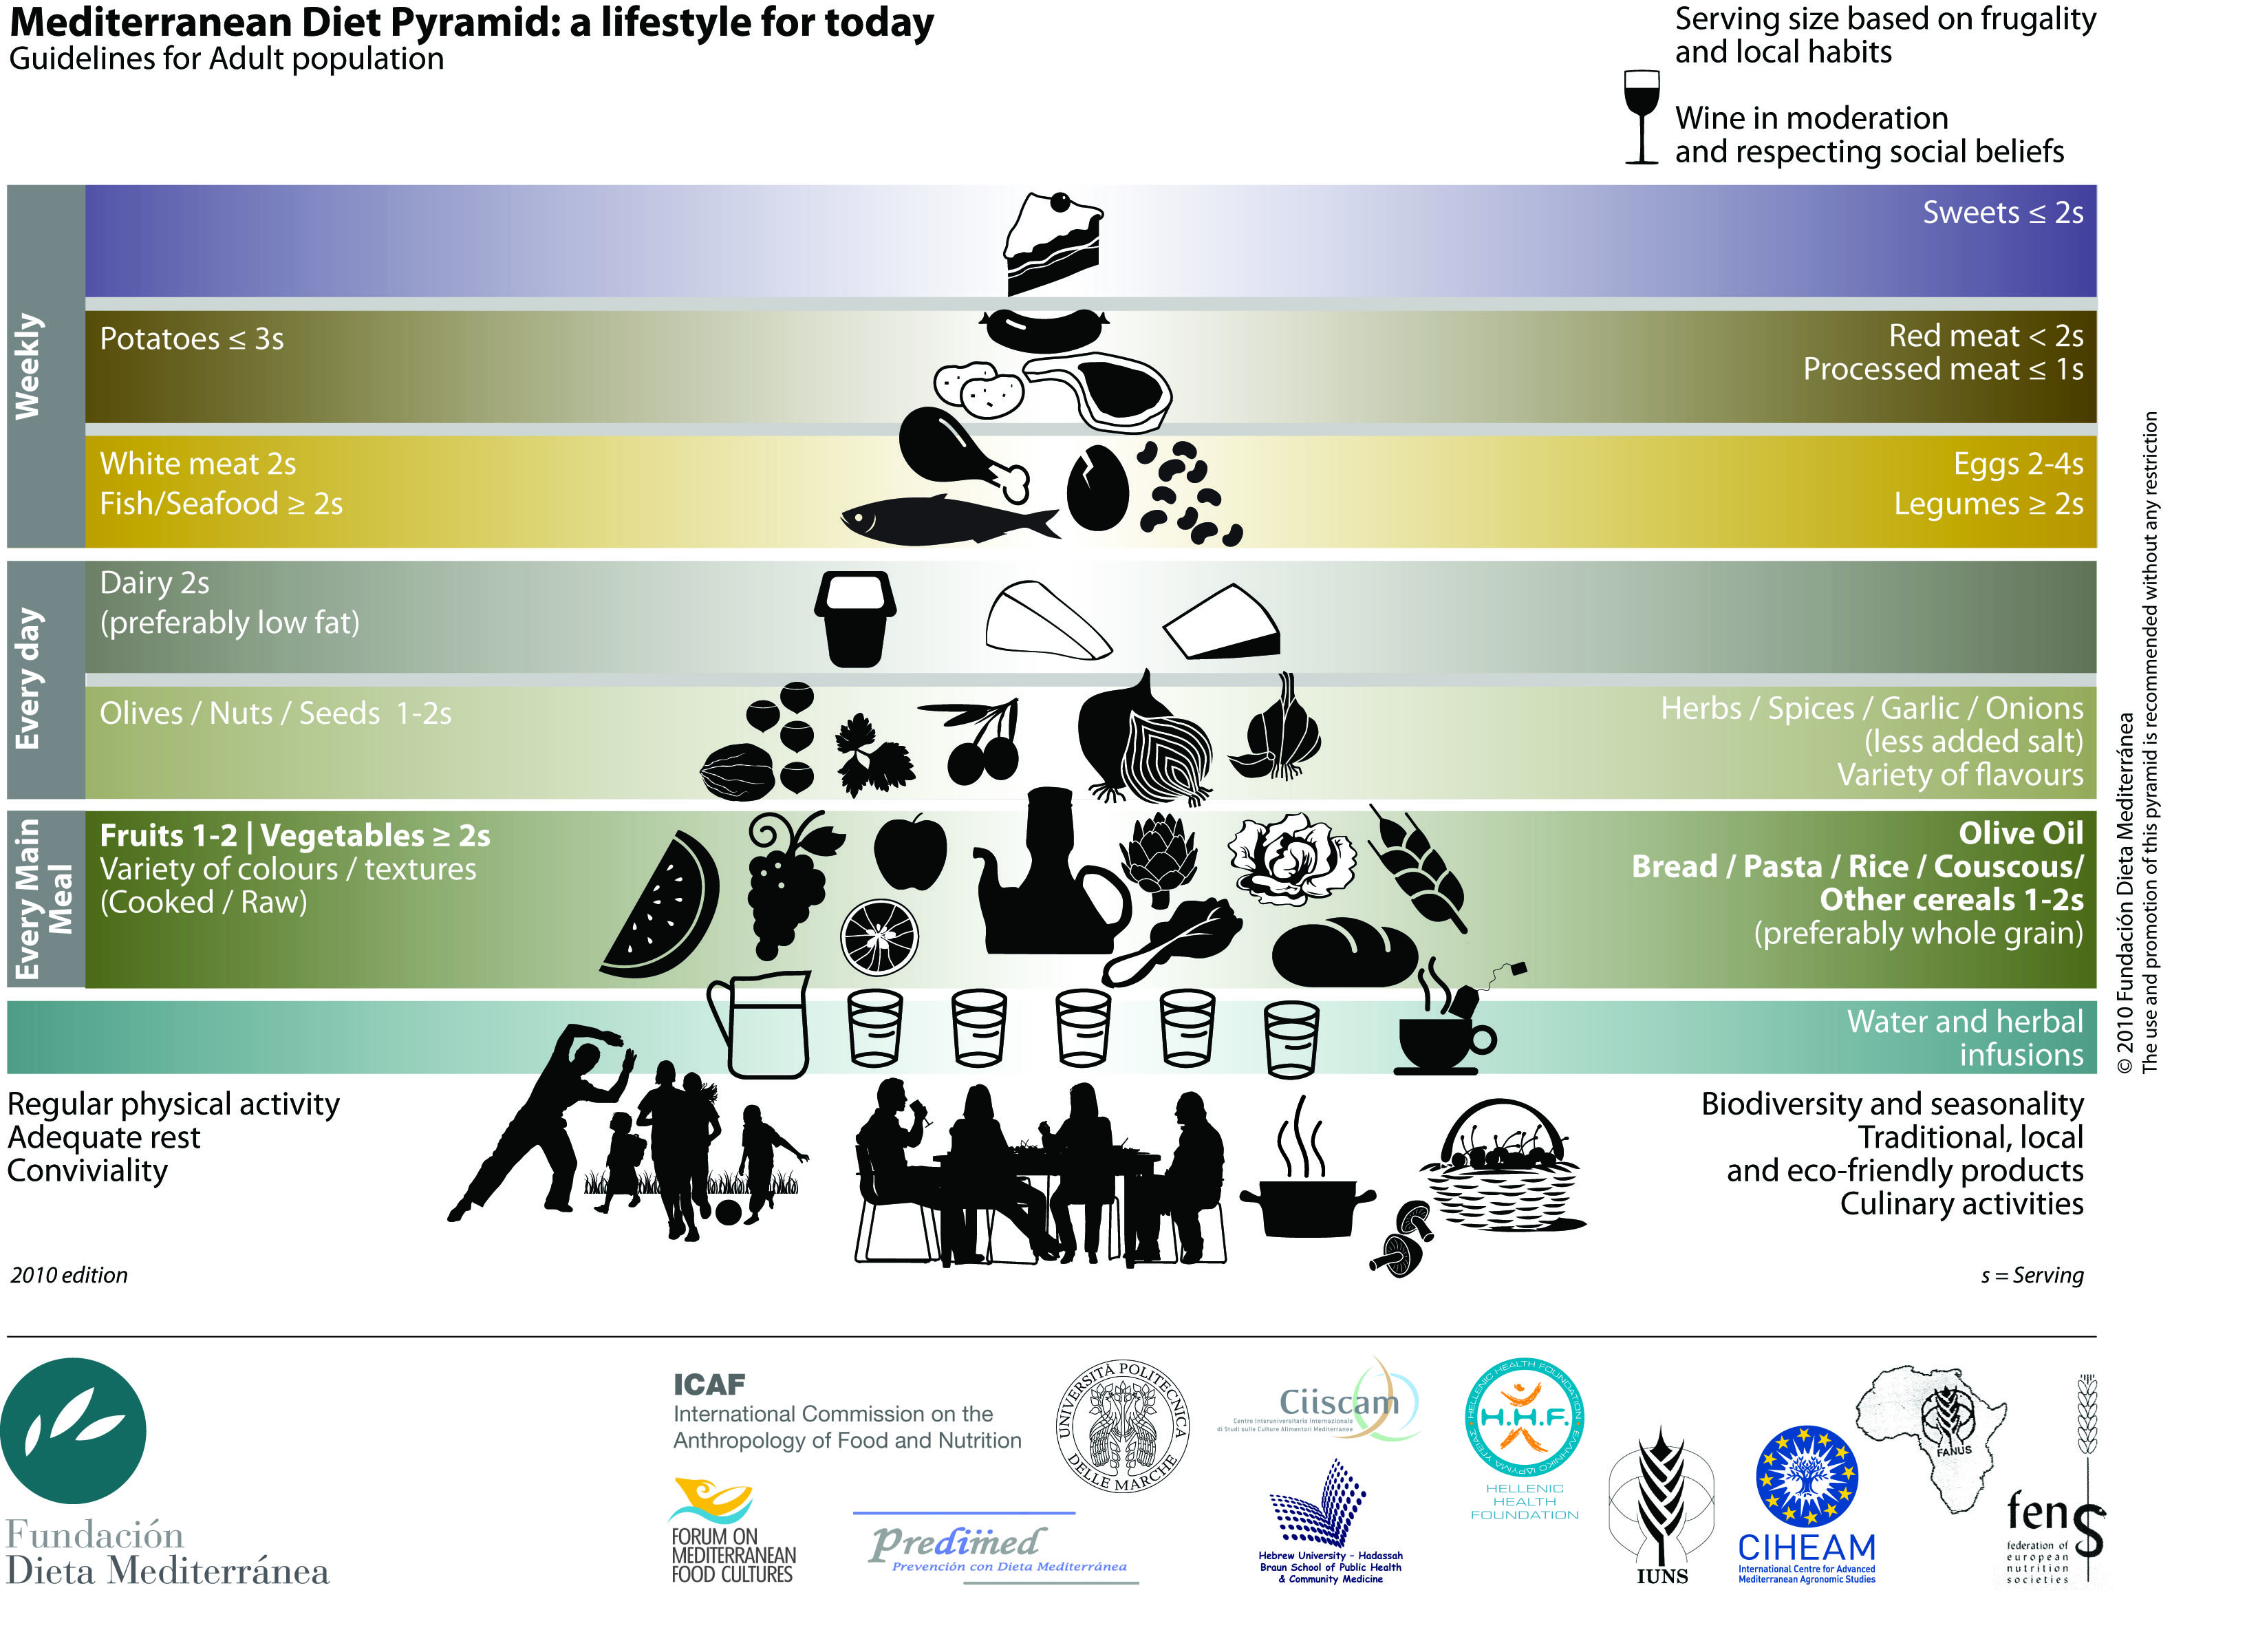
\includegraphics[scale=0.13, angle=0]{Files/prevention-study-1/figures/md-pyramid}
    \caption{The Mediterranean Diet Pyramid}
    \medskip
	\small
	As recommended by \cite{Bach-Faig2011}, who encourage use of this image without restriction.
    \label{fig: med-diet-pyramid}
\end{figure}

\textbf{Obesity.}
Within the body of literature relating to AD risk, it is apparent that obesity is interrelated with various other risk factors, including hypertension, diabetes, hyperlipidaemia and high-cholesterol \cite{Gustafson2012, Gustafson2008}. The role of excess adipose tissue and cognitive decline is not fully understood, however it is presumed to influence brain health via varied biological mechanisms \cite{Gustafson2012}.

\textbf{Fat Intake.}
During the literature review it was found that experts did not name fat intake as a specific risk factor \cite{Deckers2015}. Consumption of unsaturated fats, including omega-3 fatty acids which are found in nuts and fish, have been associated with a reduced risk of dementias \cite{Sydenham2012,Huhn2015} and is in accordance with the recommendations of the Mediterranean diet.

\subsubsection{Cognitive}
It is perhaps instinctual that the brain, like any other body-part, should be exercised in order to remain healthy and agile. As such, it is believed that exposure to cognitively stimulating or novel activities, such as those found in a complex work environment may protect against cognitive decline \cite{Roberts2014}. Studies on the subject have shown that high childhood school performance is protective of dementia risk, especially if the person continues to work in a complex work environment in adulthood \cite{Dekhtyar2015}. Therefor, it is now believed that increased cognitive activity may delay cognitive decline by increasing an individual’s cognitive reserves \cite{Sattler2012, Dekhtyar2015}.

Commercial entities have promoted the use of brain training games and apps to build a cognitive reserve \cite{Worland}. The scientific evidence on such activities is sparse and according to the editor of \textit{Cerebrum - the Dana Forum on Brain Science}:
\begin{displayquote}
``Few topics in the world of neuroscience evoke as much debate as the effectiveness of cognitive training" \cite{Boot2014}.
\end{displayquote}
The ACTIVE (Advanced Cognitive Training for Independent and Vital Elderly) trial found that cognitive training had no effect on dementia risk after as \cite{Unverzagt2012}. Despite this, the experts in a systematic review of evidence by \citeauthor{Deckers2015} ranked cognitive activity as the 3\textsuperscript{rd} most important risk factor in their Delphi rounds. Similarly, \cite{Bavelier2013} called for a collaboration between these commercial entities and the next generation of neuroscientists, to truly leverage the opportunities provided by technology.

\subsubsection{Sleep}
There have been many studies on sleep and health outcomes. In the area of dementia, there have been a number of observational studies, using objective sleep measures (e.g., polysomonography and wrist actigraphy) and self-reporting, that support links between disturbed sleep and cognitive decline \cite{Spira2014}. An observational study of 18,631 twins found a relationship between poor sleep and life dissatisfaction, leading to increased risk of stress and depression \cite{Paunio2009}. These compounding factors are discussed further in Section \ref{target-stress}. This accumulation of poor sleep also leads to day-time sleepiness, which in a 3-year longitudinal study with 1041 participants was found to be a statistically significant independent risk factor for dementia in older adults \cite{Tsapanou2015}.
From the literature it appears that healthy sleep plays an important role in maintaining brain health in ageing \cite{Spira2014}, and an effort to improve sleep quality by minimising disturbances could potentially play a key role in dementia prevention.

\subsubsection{Stress} \label{target-stress}
The effects of stress include hypertension, depression and disturbed sleep \cite{Schneiderman2005}. Each of these have a documented relationship with AD risk. It is known that depression plays a role on executive functioning and is associated with the onset of dementias in later life \cite{Dotson2010,Royall2012,Boyle2010}. Hypertension is present in all major causes of cognitive impairment \cite{Iadecola2014}. The relationship is not fully understood, however, potential mechanisms include focal brain atrophy, ischemia, white matter disease and Amyloid accumulation \cite{Iadecola2014}. Many placebo-controlled trials aiming to lower blood pressure have been performed, which have shown positive and desirable effects \cite{Staessen2011}. These trials were performed with subjects in later life, and the results were inconclusive as to whether lowering blood pressure can \textit{reverse} Alzheimer's disease risk.

\subsubsection{Social}
Greater levels of social engagement and participation are associated with lower rates of dementia \cite{Saczynski2006, Fratiglioni2000}. An analysis of 2089 subjects, followed over 15 years showed that it is the quality of these social relationships that is the most important factor \cite{Amieva2010}. As relationship satisfaction and reciprocity increased, dementia incidence decreased \cite{Amieva2010}. These findings may be explained due to increased cognitive stimulation, and a reduced risk of depression \cite{Saczynski2010}.

\subsubsection{Smoking}
Smoking comes with a plethora of health risks, including an increased risk of dementias \cite{cdc_smoking}. \citeauthor{Deckers2015} noted 13 studies on smoking and dementia risk, of which 10 found increased risk \cite{Deckers2015}. Experts rated smoking as the 8\textsuperscript{th} most important factor regarding AD risk as part of their Delphi analysis of existing evidence. Further analysis of these studies showed that current smokers have a 59\% increased risk of developing AD \cite{Peters2008}. As with many neurological conditions, the exact mechanisms behind the association are still unknown.

\subsubsection{Summary of Key Measures}
It is possible to quantify behaviour in each domain by monitoring key measures. Table \ref{tbl: key-measures} describes the key measures which were developed from the literature review. Many domains have more than one key measure, as many are multifaceted and complex. Note that the social domain only has one measure, which is a subjective rating of social engagement and does not measure an objective measure, such as time spent in social scenarios. This is due to the finding that quality of social relationships and interactions are the most important factor \cite{Amieva2010}.

\begin{table}[h]
\centering
\caption{Key Behaviour Measures for AD Behaviours}
\label{tbl: key-measures}
\resizebox{\textwidth}{!}{ %Resizes the box to fit all text
\begin{tabular}{@{}llll@{}}
\toprule
Domain                     & Measure                               & Unit         & Type       \\ \midrule
\multirow{2}{*}{Cognitive} & Time spent on New/Novel activities         & minutes      & objective  \\
                           & Time spent on Stimulating activities         & minutes      & objective  \\ \midrule
\multirow{3}{*}{Diet}      & Consumption of  fruits and vegetables       & cups         & objective  \\
                           & Consumption of whole grains                 & ounces       & objective  \\
                           & Consumption of nuts, seeds, or legumes      & servings     & objective  \\ \midrule
\multirow{2}{*}{Physical}  & Time spent doing moderate physical activity & minutes      & objective  \\
                           & Time spent doing vigorous physical activity & minutes      & objective  \\ \midrule
\multirow{3}{*}{Sleep}     & Rate effort to promote sleep                & rating-scale & subjective \\
                           & Self-rate sleep quality                     & rating-scale & subjective \\
                           & Duration of sleep                           & hours        & objective  \\ \midrule
Social                     & Rate social engagement                      & rating-scale & subjective \\ \midrule
\multirow{2}{*}{Stress}    & Self-rate stress level                      & rating-scale & subjective \\
                           & Effort to decrease stress                   & rating-scale & subjective \\ \bottomrule
\end{tabular}
}%end of resize
\end{table}

\subsection{Development of Delivery Mechanism and Tracking Tools}

Adopting a modular approach to the design and development of the platform enables components of the system to be added, removed or re-used in other similar systems. Given that the preparation, action and maintenance phases of the TTM consist of numerous process, it is appropriate that a platform intending to supplement behaviour change can address each of these processes in a modular fashion. For the purpose of reducing AD risk, the following components were identified as being necessary:
\begin{itemize}
\item \textbf{Education} about AD risk and prevention strategies.
\item \textbf{Monitoring} relevant behaviours through observation or self-reporting.
\item \textbf{Feedback} provision based on observed behaviours and targets.
\end{itemize}

Using a tab-based user interface (UI) each identified component is displayed to the user as a separate tab, helping separate their functions and reducing the overlap of content and behaviour change strategies.

\subsection{Education Component}
To assist users in their traversal of the TTM, education plays a key role to support motivations and efficacy in reaching set goals. As the identified platform is mobile, the intended users are in need of a method to receive information in a succinct and efficient manner.

\subsubsection{Daily Facts}
For each of the core domains and associated risk factors identified in Table \ref{tbl: behavioural domains},  numerous prevention methods were identified from medical literature, and further developed by a team of psychologists, epidemiologists and nutritionists at Utah State University \cite{Norton2015-TRCI}. These risk factors and their associated prevention methods were translated into layman's terms. Each identified risk factor or behaviour was assigned one or more suggestions, thereby creating over 160 fact and suggestion pairs. These pairs are hereafter referred to as daily facts. The quantity of the daily facts are reflective of the supporting medical literature and are summarised in Table \ref{tbl: daily fact count}. An example daily fact from the diet domain is as follows: \textit{“Consuming high amounts of processed foods is related to cognitive decline\ldots Try a fresh salad for dinner instead of something from a box”}.
\begin{table}
\centering
\caption{Number of daily facts for each behavioural domain}
\label{tbl: daily fact count}
\begin{tabular}{@{}l c@{}}
\toprule
Domain    & Number of Daily Fact Pairs \\ 	\midrule
Physical  & 23                              \\
Diet      & 66                              \\
Sleep     & 14                              \\
Cognitive & 24                              \\
Stress    & 10                             	\\
Social    & 27                              \\ \hline \hline
Total	  & 164								\\	\bottomrule
\end{tabular}
\end{table}

\subsubsection{Presentation of daily facts}
Information presented visually on a screen is processed differently than verbally from a person \cite{Sundar2015}. Avatars have been used extensively to facilitate the mediation of information in computer-user interactions. Their use includes user-to-user communications, social media, advertising, news-reports and job interviews \cite{Sundar2015}. The avatar acts as a visual representation of the knowledge source \cite{Bente2008} and are hypothesised to enhance social interactions \cite{Blascovich2002}. Therefore, they are also expected to increase trust in communications. Additionally, the use of certain visual characteristics of an avatar can have an effect on the rational choice that the user has on the information presented. These choices include assessing the level of uncertainty in the information  source \cite{Afifi2000}. As such, for this particular use-case a number of personas were considered to represent the knowledge source of the daily facts \cite{Sundar2015}, to best increase trust in the information presented. These included a doctor, a nurse and a coach. Relying on expert advice from psychologists at Utah State University, the coach was identified as the suitable avatar and can be seen in implemented within the app in Figure \ref{fig: screenshot-dailyfact}.

\begin{figure}[h]
    \centering
    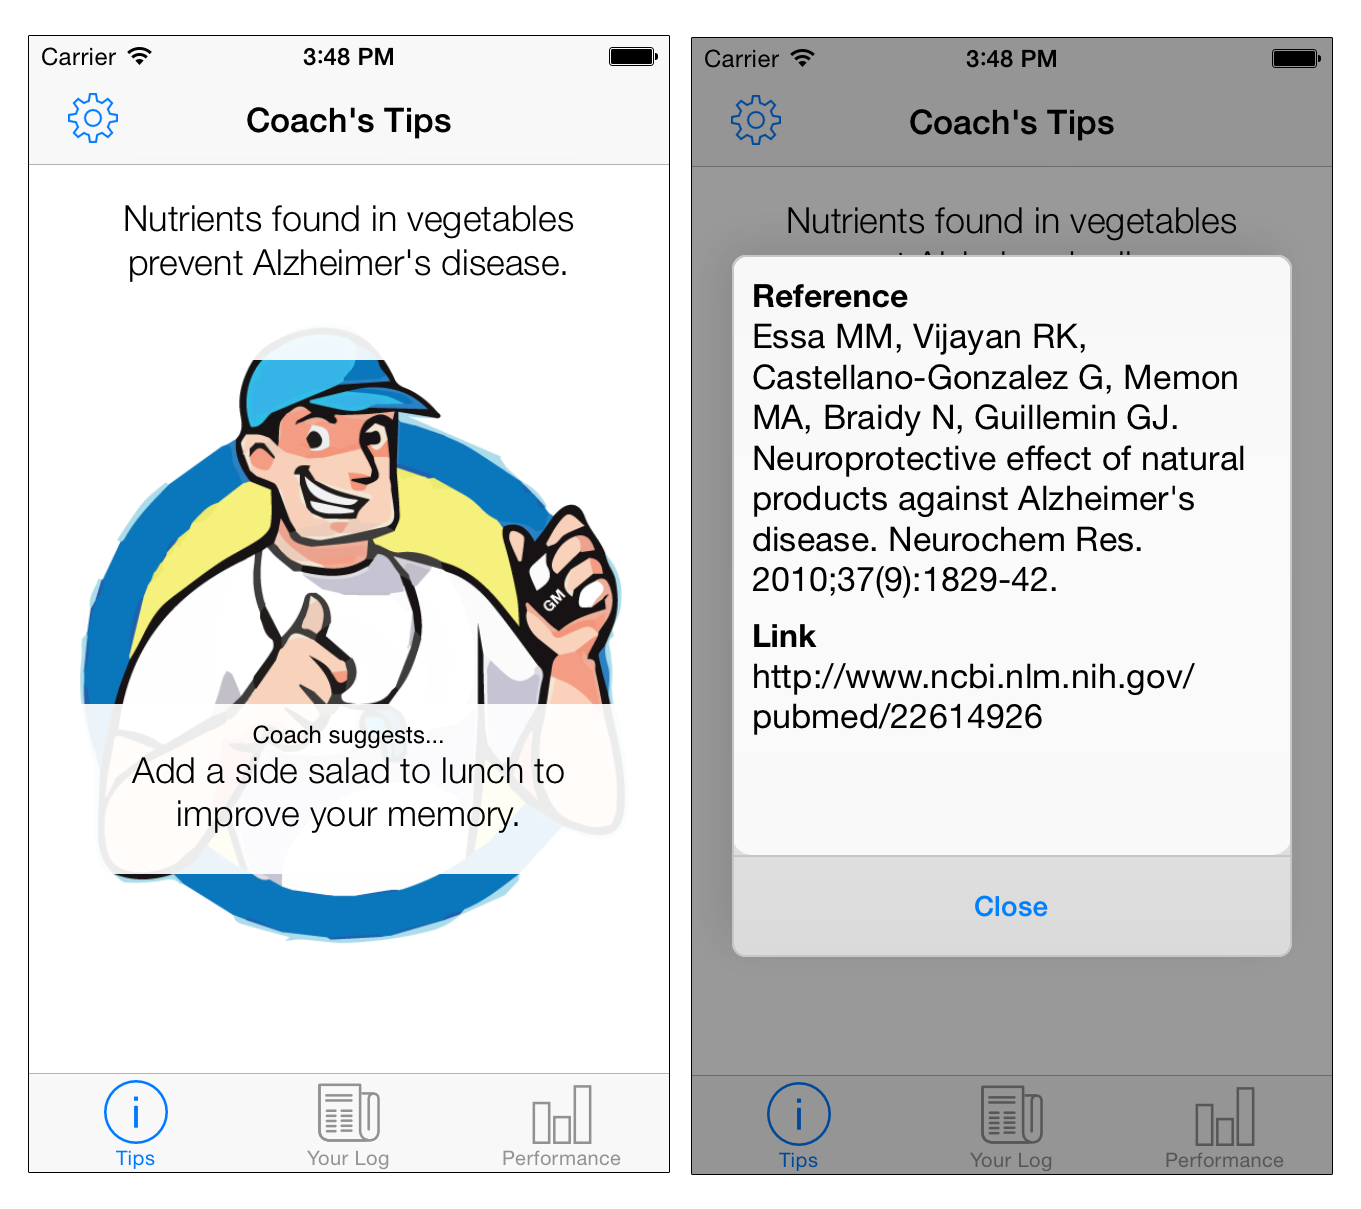
\includegraphics[scale=0.25, angle=0]{Files/prevention-study-1/figures/screenshot-dailyfact.png}
    \caption{Screenshot of app showing daily fact with supporting literary evidence}
    \label{fig: screenshot-dailyfact}
\end{figure}

\subsubsection{Learning favourable behaviours}
To assess behaviour change for each domain, a number of questions are designed to be presented to the user each day (specific information for each question is detailed in Section \ref{subsection-montoringcomponent}). In addition to being a method to gain insight into user behaviours, the questions also aim to educate about the quantity and quality of certain behaviours through self-assessment. Users can view what the recommended target is for each behaviour type, report their own behaviour and immediately understand their relative performance. Through this repetitive daily process, users become educated about ideal targets and methods to achieve them.

\subsection{Monitoring Component} \label{subsection-montoringcomponent}
The monitoring component of the app is designed to allow the user to perform various processes of the TTM, including consciousness raising, self-re-evaluation and reinforcement management. For an individual to effectively modify their behaviour, they should understand what their current behaviour is and what their ideal or target behaviour should be. To do this, the app provides a mode which allows the user to report their behaviours relevant to AD risk on a daily basis.

\subsubsection{Facilitating self-reporting}
For each of the identified domains, daily questions were developed and refined from the list of key measures (Table \ref{tbl: key-measures}), to capture behaviours relevant to AD risk. All questions were quantitative in nature, however, contained a mixture of subjective and objective questions. For example, a user may be asked to report the number of fruits and vegetables they consumed in a day (objective), and also rate their quality of sleep on a scale of 0-10 (subjective).
In addition to the questions for the original 6 behavioural domains, a question was added to collect any activity data observed via a user's wearable activity monitor. In total 12 questions were designed for the domains: Physical (2), Diet (3), Social (1), Sleep (1), Cognitive (2) and Stress (2) and Wearable Activity Monitor (1). For each question, a recommended daily target value was extracted from external knowledge sources, such as the World Health Organisation (WHO), the American Heart Foundation (AHF), and the Centre for Disease Control and Prevention’s (CDC). Full details of these questions can be seen in Table \ref{tbl: questions}.

\begin{sidewaystable}[ph!]
\centering
\caption{Questions presented to the user, showing their minimum, maximum and recommended values}
\label{tbl: questions}
\resizebox{23cm}{!}{%  begin resize to fit text
\begin{tabular}{lllllll}
\toprule
Domain                     & Id & Question                                                                         & Min. & Max. & Recommended     &  \\ \midrule
\multirow{2}{*}{Cognitive} & 1  & How many minutes did you spend today doing ``novel mental exercises''?             & 0    & 120  & 30 minutes      &  \\
                           & 2  & How many minutes did you spend today doing ``cognitively stimulating activities''? & 0    & 120  & 30 minutes      &  \\ \midrule
\multirow{3}{*}{Diet}      & 3  & How many cups of fruits and vegetables did you eat today?                        & 0    & 10   & 5 cups          &  \\
                           & 4  & How many ounces of whole grains did you eat today?                               & 0    & 10   & 3 ounces        &  \\
                           & 5  & How many servings of nuts, seeds, or legumes did you eat today?                  & 0    & 5    & 1 serving       &  \\ \midrule
\multirow{2}{*}{Physical}  & 6  & How many minutes of ``moderate'' physical activity did you do today?               & 0    & 60   & 30 minutes      &  \\
                           & 7  & How many minutes of ``vigorous'' physical activity did you do today?               & 0    & 60   & 20 minutes      &  \\ \midrule
Sleep                      & 8  & How would you rate your sleep promotion efforts over the past 24 hours?          & 0    & 5    & 5 (out of 5)    &  \\ \midrule
Social                     & 9  & How would you rate your social engagement in the last 24 hours?                  & 0    & 7    & 7 (out of 7)    &  \\ \midrule
\multirow{2}{*}{Stress}    & 10 & How much effort have you put into decreasing your stress over the past 24 hours? & 0    & 10   & 10 (out of 10)  &  \\
                           & 11 & On a scale of 1-10 how would you rate your stress level over the past 24 hours?  & 1    & 10   & 1 (out of 10)   &  \\ \midrule
Wearable                   & 12 & How many Nike Fuelpoints did you earn today?                                     & 0    & 5000 & 2000 Fuelpoints &  \\ \bottomrule
\end{tabular}
} % end resizebox
\end{sidewaystable}

The recommended value serves 3 key purposes:
\begin{enumerate}[noitemsep,topsep=0pt]
\item to act as an \textbf{observable goal} for the user.
\item to efficiently \textbf{calculate performance} of a user.
\item to \textbf{compare performances} of other users.
\end{enumerate}

Further information of calculating performance is detailed in Section \ref{subsubsection-calculating-performance}.

\subsubsection{Data Entry}
Data entry for each question is facilitated by a bespoke list view, that uses a draggable sliding bar to allow quick and accurate entry of information. A screenshot of the listview containing several questions can be seen in Figure \ref{fig: screenshot-measure}. Each list item contains a fixed-width slider bar, with a draggable circle that moves on the horizontal plane. As the circle moves from left-to-right, the value increments by a set value, typically by 1. Displaying progress as a bar that grows on the horizontal plane gives the user immediate visual feedback toward their current progress. The maximal value achievable for each slider is typically double the recommended value, allowing users to overachieve their targets and give recognition to their efforts (reinforcement-management).

\begin{figure}[h]
    \centering
    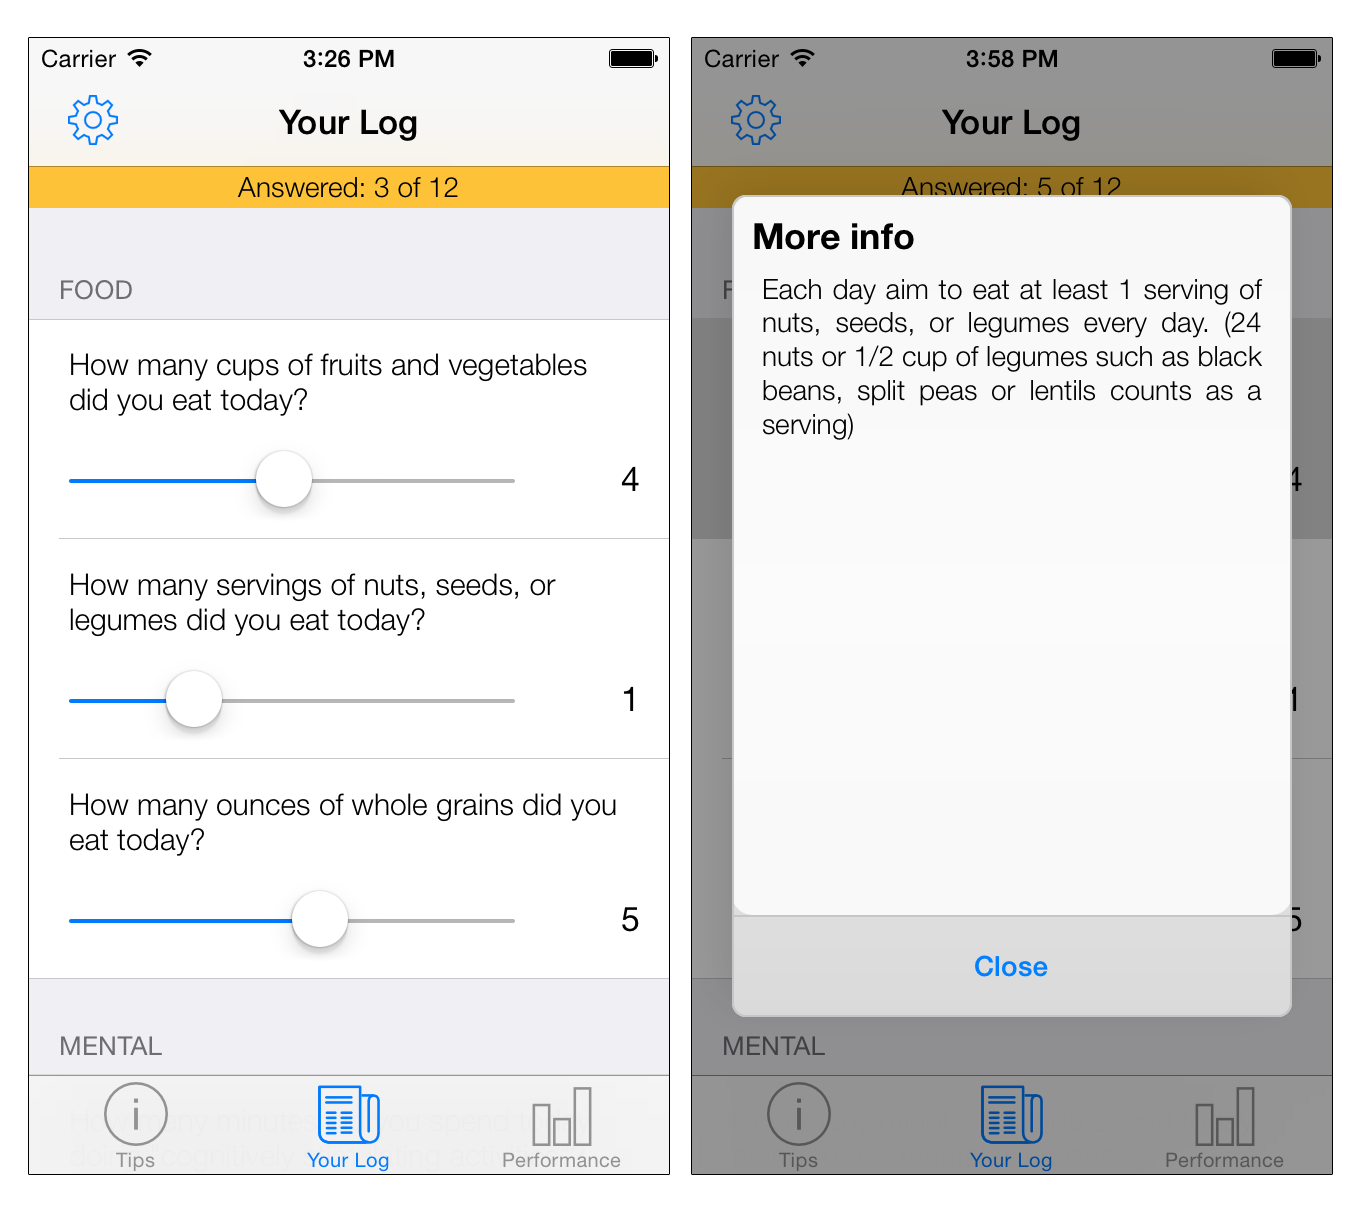
\includegraphics[scale=0.25, angle=0]{Files/prevention-study-1/figures/screenshot-measure.png}
    \caption{Screenshot of app showing self-reporting screens and supporting information}
    \label{fig: screenshot-measure}
\end{figure}

\subsubsection{Improving Question Interpretation}
To assess behaviour change for each domain, a number of questions are designed to be presented to the user. Each question seeks to measure information about a user's behaviours longitudinally, both in a qualitative and quantitative manner. In order for these measurements to remain accurate, the user must understand what the question is asking, how they can measure it, and what the favourable result is. Therefore, the user must be educated on the topic to which they are being queried.
For example, the question:
\begin{displayquote}
``How many servings of nuts, seeds, or legumes did you eat today?"
\end{displayquote}
may elicit confusion for a number of reasons. Firstly, the user may not know the existence of certain aforementioned food items. Secondly, the user may also be unsure of what constitutes a \textit{`serving'} of the items, or how many servings are favoured.
To address these issues, the app provides descriptions of all of these areas which may lead to potential uncertainty for the user. Ensuring that all users understand the question is vital for comparisons of self-reported behaviours across multiple users. An example of additional information regarding a specific question can be seen in Figure \ref{fig: screenshot-measure}.

\subsection{Feedback Component}
The feedback component of the app is designed primarily to motivate the user through to self-re-evaluation, reinforcement management and also via established gamification techniques.

\subsubsection{Gamification}
Motivation plays a key role in all models of behaviour change. Maintaining motivation is difficult over time, and may people relapse to their prior behaviours, simply because they no longer feel motivated to progress. Gamification involves turning typically mundane tasks into a form of game, utilising a variety of methods commonly found in game playing, such as points earning, competition and reward systems \cite{Deterding2011a}. All of these game mechanics have been found to encourage continual engagement, and subsequently progression in various studies \cite{Hamari2014}. Gamification is a relatively new concept, and its use to encourage behaviour change in adults is relatively limited. However, initial findings show that it can be applied successfully in health care promotions to maximise engagement \cite{Schoech2013}. Therefore, within this mobile app, points earning elements of gamification have been implemented as a mechanism by which users may be encouraged to achieve their daily recommended targets.

Upon entering data for a question, the user can view their relative performance for that domain in the performance tab. Each topic is shown in a listview, accompanied by a number of achievable stars. The stars are designed to encourage and reinforce a participant’s effort to change their behaviour. Since all domains can be viewed on screen at the same time, it provides a fast method to deliver visual feedback on the domains that require more effort, and which are under control \cite{Hartin2015-JMIR}. This can be seen in Figure \ref{fig: screenshot-performance}.
\begin{figure}[h]
    \centering
    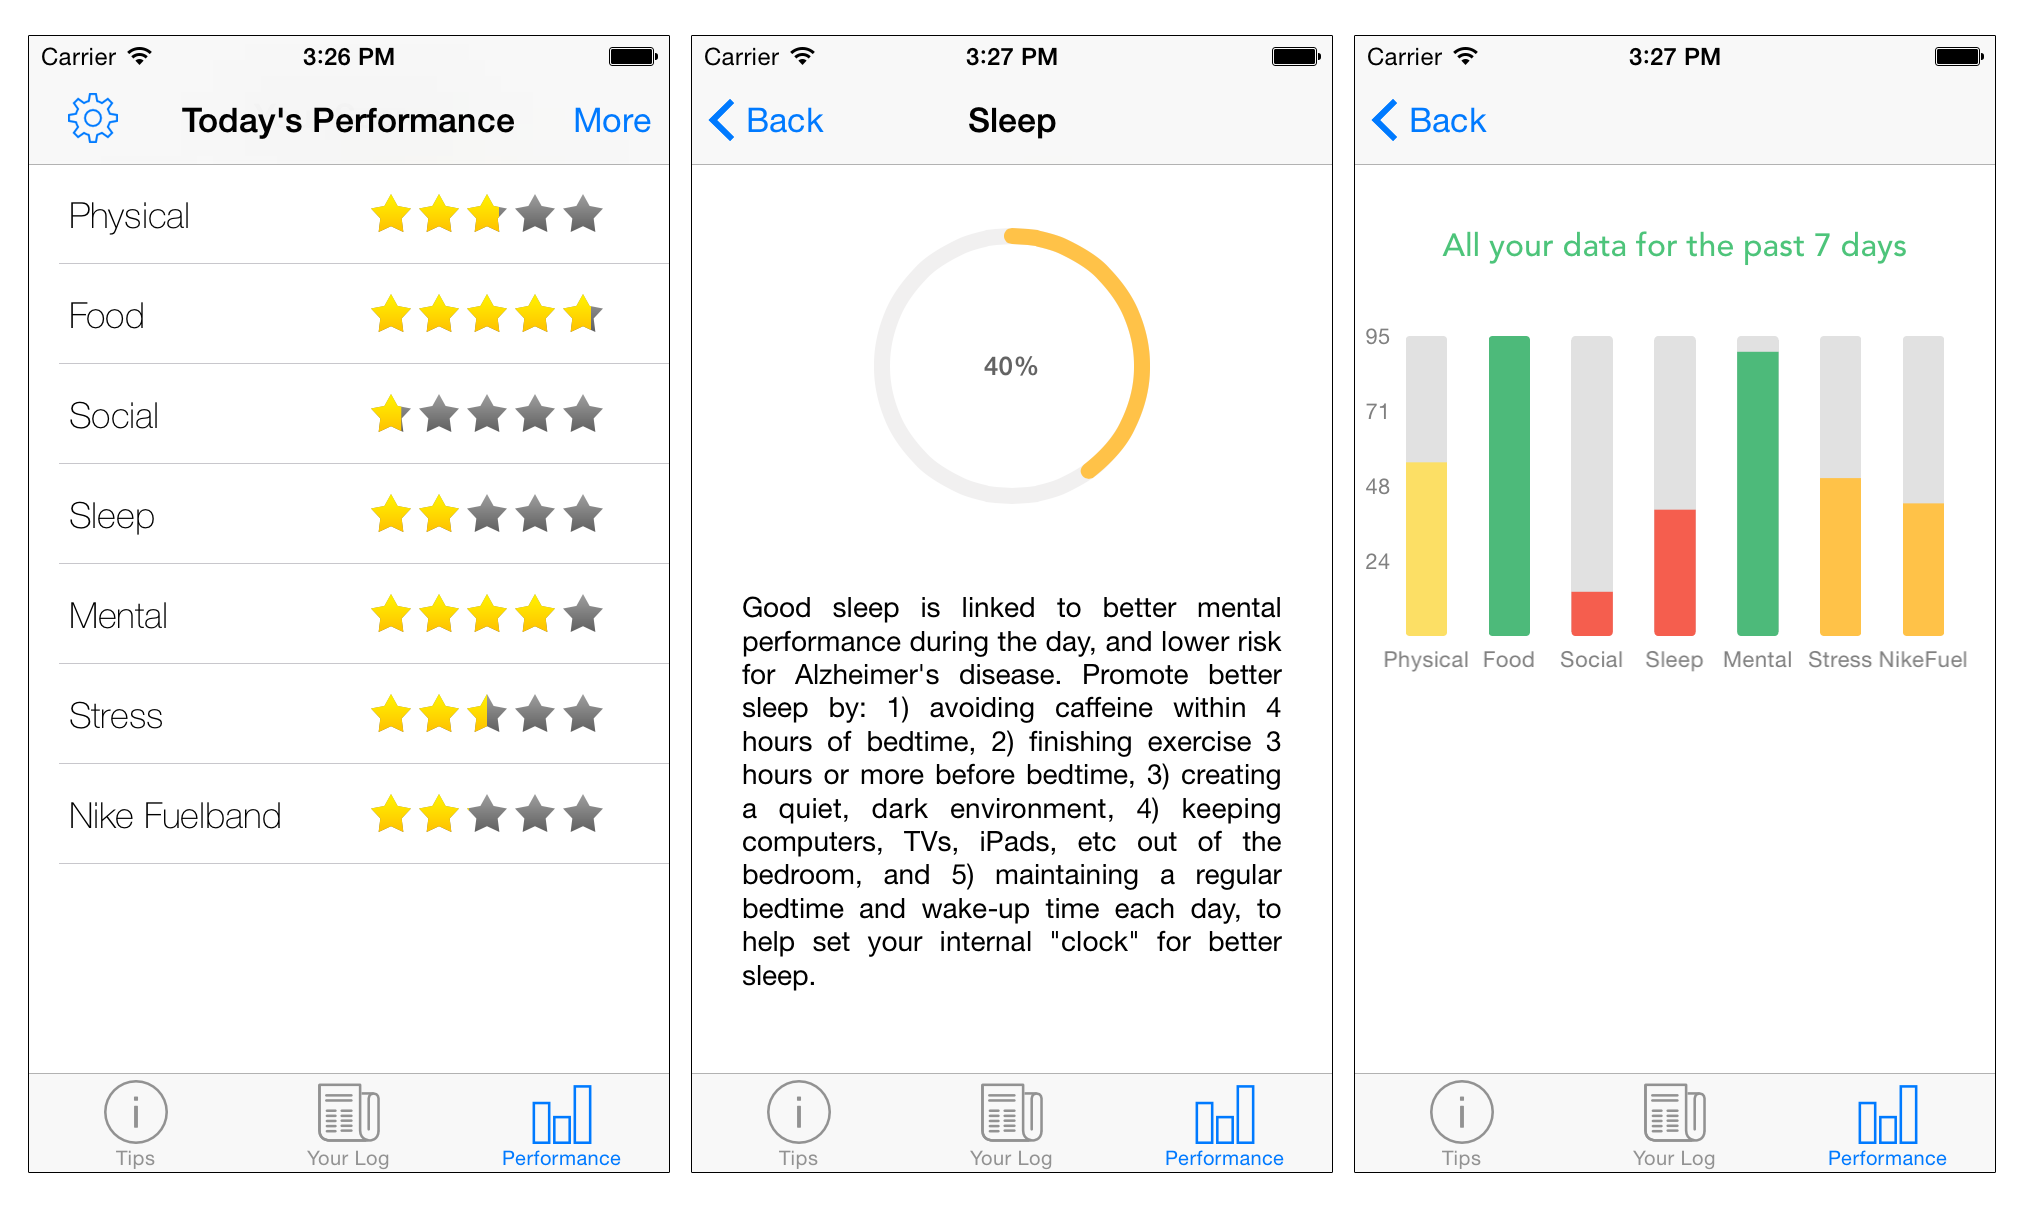
\includegraphics[scale=0.2, angle=0]{Files/prevention-study-1/figures/screenshot-feedback.png}
    \caption{Screenshots of app showing high-level and longitudinal feedback on reported behaviours}
    \label{fig: screenshot-performance}
\end{figure}

Users may also tap upon each domain to display an information screen, providing additional pertinent material about that domain with a further graphical representation of their efforts. In this same screen, users are provided with additional tips and methods by which they could improve their performance. For example, in the sleep domain, tips include:
\begin{enumerate}[noitemsep,topsep=0pt]
\item Avoid caffiece within 4 hours of bedtime.
\item Keep computers, TVs, iPads etc, out of the bedroom.
\item Maintaining a regular bedtime and rise time each day will help set your internal clock for better sleep.
\end{enumerate}

All tips and further information developed can be seen in Appendix \ref{apndx: domain-tips}.

The users may also view their performance aggregated across the previous 7 days in the form of a bar chart or spider diagram. Again this serves to visually assist the participants in understanding their behaviours longitudinally for the purpose of self-affirmation and reinforcement management, discussed in the processes of the TTM.

\subsubsection{Calculating Performance} \label{subsubsection-calculating-performance}
Using the concepts explored in gamification, the user can achieve a maximum of 5 stars for each behavioural domain each day. To receive the full 5 stars for a domain, the user must achieve the recommended values for all the behaviours within that domain (See Table \ref{tbl: questions}). Since many of the behaviours are reported across various fixed value ranges, the values must be normalised to within a range of 0 - 5 in relation to the recommended value \cite{Hartin2014-IWAAL}. This is achieved within the app via the following function
\begin{equation}
f(x) = \left\{
         \begin{array}{l l}

         R_{U} & \quad
           \text{if }{x \geq Q_{G} }\\

           \frac{
           \left(x-Q_{L}\right)\times\left(R_{U}-R_{L}\right)}
           {Q_{G}-Q_{L}}
           + R_{L} & \quad
           \text{if }{Q_{L} \leq x < Q_{G}}\\

          \end{array}
          \right.
          \label{eq: calc-performance-stars}
\end{equation}

where $x$ is the user’s answer value to a particular question, $Q_{G}$ is the goal value for the question, $Q_{L}$ is the lowest possible value for that question, $R_{U}$ is the upper boundary of the normalised result and $R_{L}$ is the lowest boundary.

\subsection{Usage Component}
This component of the framework involves the monitoring of the users interactions with the app for the benefit of the developers and health investigators.
Using a mixture of proprietary and open-source analytical tools \cite{Hartin2014-IWAAL,GoogleAnalyticsWeb,MixpanelAnalytics}, it is possible to inject traceable hooks into any aspect of the apps code base. Within this app, the following actions were identified to be tracked via analytic code:
\begin{itemize}[noitemsep,topsep=0pt]
\item Launching the app.
\item Navigating screens.
\item Updating behaviours.
\item Seeking additional detail for topics/questions.
\item Seeking additional detail for performance.
\item Changing notification times.
\end{itemize}

Observing these actions will allow the developer to further understand the needs of the end-user without direct communication. This can be performed in a number of ways: by measuring which actions are the most commonly used within the app, observing the typical screen flow of users and assessing if users are getting stuck at specific points in the app.
Additional useful information can be gleaned by combining this app usage data, with the behavioural data reported by the user. From this combination, observations can be made to establish which user, or user types, benefit most from the system in its current version and also identify those who may require additional support.

\subsection{Data Component}
This data component controls the storing and uploading of the users behaviours, both self-reported and extracted from app usage for the benefit of the health investigators. Health investigators, those facilitating the behaviour change intervention, are interested in observing trends, making predictions and detecting anomalies. Therefore, the integrity and accessibility of the data is vitally important to this party, particularly if analyses are to be carried out mid-intervention. The networking model implemented for this framework is centralised client-server model, whereby a number of clients access a single networked server. This is illustrated in Figure \ref{fig: clientserver-model}.

\begin{figure}[h]
    \centering
    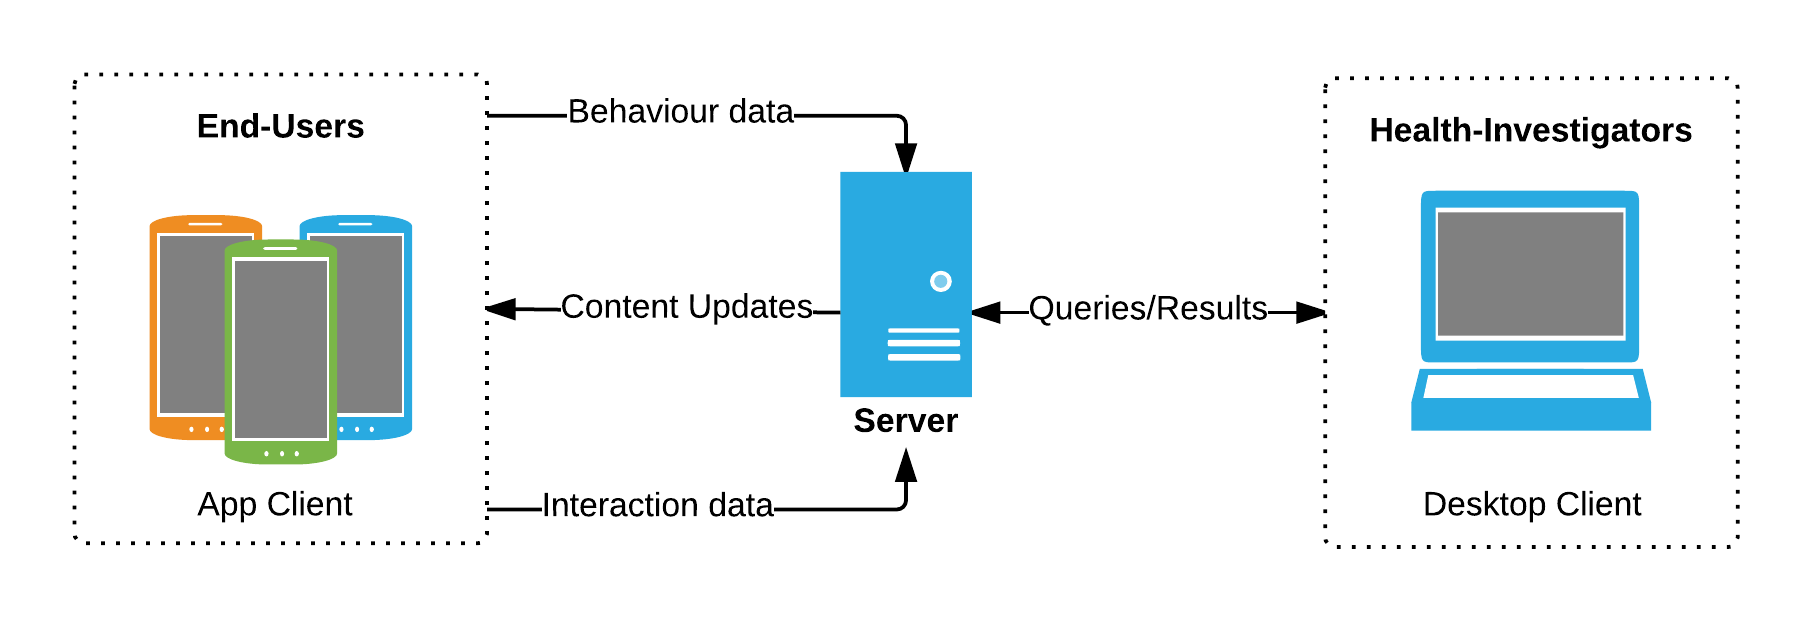
\includegraphics[scale=0.9, angle=0]{Files/prevention-study-1/figures/client-server}
    \caption{Centralised Client-Server Network Model}
    \label{fig: clientserver-model}
\end{figure}

\subsubsection{Uploading Data}
Upon installation of the app on a smartphone, a local database is created to contain app specific data. This data is intermittently uploaded to the central server. Data only flows between the client (app) and the server. Data cannot be directly shared between clients, i.e. from one installation of the app to another, without first being processed and authenticated by the central server (Further detail regarding protocols are discussed in Section \ref{subsection-api}).

\subsubsection{Downloading Data}
Since the scientific evidence is forever evolving on AD risk factors and prevention methods, the information that the app is packaged with should not be considered final. All information displayed to the user via the app can be updated from the central server. This includes the daily facts, the language used in the behavioural questions, their supplementary descriptions, and the feedback text in the performance tabs. Upon a change to any of this material on the central database, a global version number is updated. The app will frequently check if its local version number matches the global version number on the central server. If an app detects that the local version number is outdated, the app will pull the changes from the server and update its local database.

\section{Business Logic Implementation}
The application server performs the majority of the business logic involved within this system, including the registration of participants, handling authentication, controlling access to the intervention material, and aggregation of participant data. The server runs a variant of the open-source linux operating system, contains a number of statistical software packages and hosts a relational database management system (RDBMS). Since the app relies heavily upon the transfer of data between client and server via the internet, an application programming interface (API) was developed to facilitate these functions through the methods outlined in representational state transfer (REST) architecture \cite{Fielding2000, Benslimane2008}. This is further illustrated at a high-level in Figure \ref{fig: clientserver-model-detail}.

\begin{figure}[h]
    \centering
    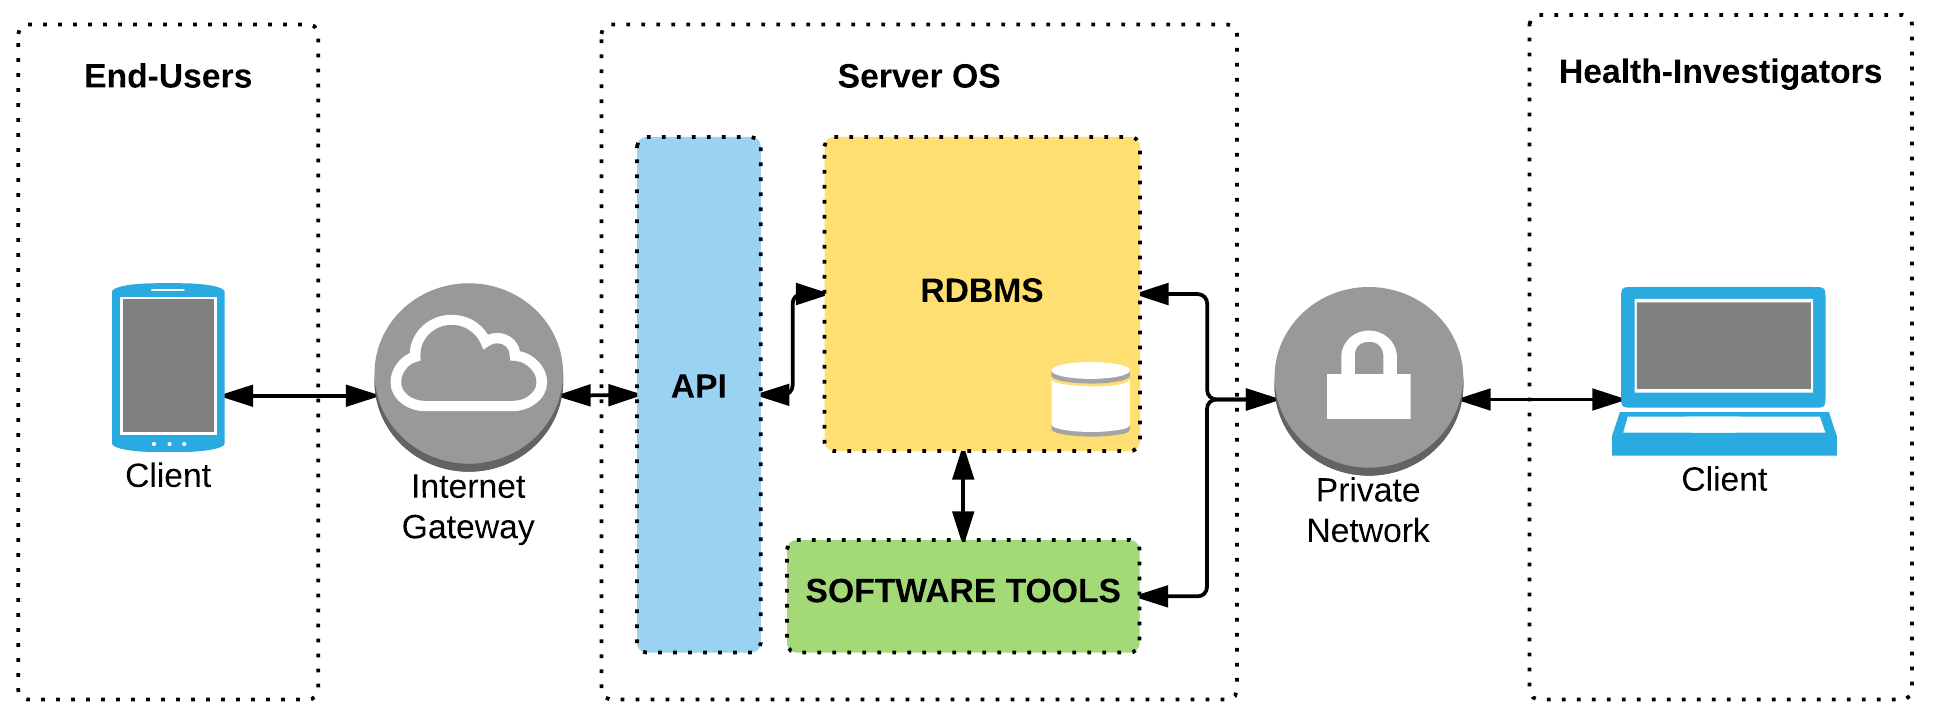
\includegraphics[scale=0.9, angle=0]{Files/prevention-study-1/figures/client-server-adapted}
    \caption{High-level Server Architecture Overview}
    \label{fig: clientserver-model-detail}
\end{figure}

\subsection{Database Schema}
The database schema describes the structure, format and relationships between the models in the RDBMS. In this system, various components of the app have been re-modelled for the act of persistence and storage on the servers RDBMS. Figure \ref{fig: database-model} shows these models in detail. Using the same models throughout the client and the server development dramatically improves development overheads, reduces the risk of type-mismatches, and enables reflection of objects across the Android and iOS platforms \cite{Thalheim2000}.
\begin{figure}[h]
    \centering
    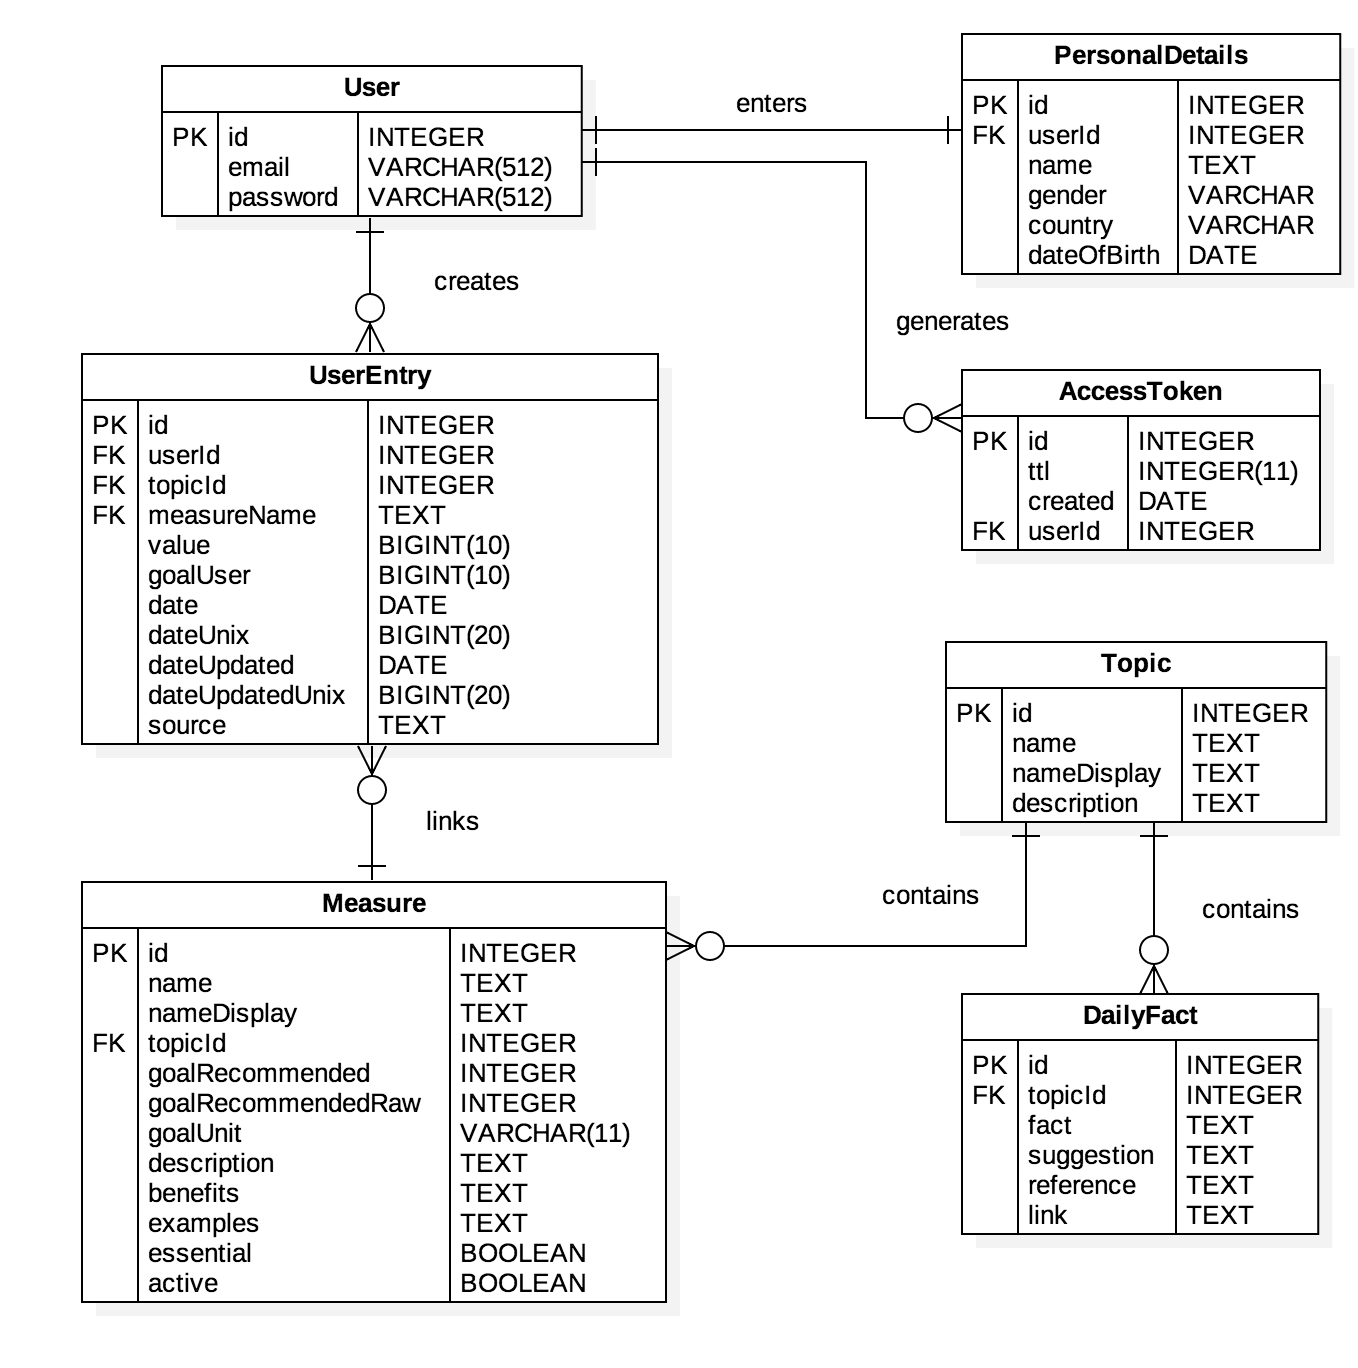
\includegraphics[scale=0.3, angle=0]{Files/prevention-study-1/figures/database-model}
    \caption{Data Model}
    \label{fig: database-model}
\end{figure}


\subsubsection{Exposing models through a RESTful API} \label{subsection-api}
With a well-defined and stable data model, it is possible to expose certain aspects of the model via an API. The creation of an API allows controlled interaction between the server and its clients, through a set of defined methods and routines. With the goal of keeping the data model intact on the central server, implementing strict protocols within the API is very beneficial. In this use-case, potential client's operating systems will be varied (iOS, Android). As such, their platform specific languages and data-models can also vary, yet the API requires that all data transmitted conforms to its protocols. Using a language independent notation, such as JSON (JavaScript Object Notation), enforces system-wide validity of transmitted data, which is of paramount importance to the health-investigators study analyses.

\subsubsection{Topics}
A Topic object is at the highest organisational level of the educational content. Each topic is identified by a unique id, which is used as a foreign key reference for its associated daily facts and measures. JSON Example: \inputminted{json}{Files/prevention-study-1/code/topicexample.json}

\subsubsection{DailyFacts}
A DailyFact object belongs to a topic, and consists of a fact and suggestion pair, with references to the supporting scientific literature and an internet enabled hyperlink. JSON Example: \inputminted{json}{Files/prevention-study-1/code/dailyfact.json}

\subsubsection{Measures}
A Measure object belongs to a topic and describes a behaviour which is being measured. This measure contains the recommended goal and its unit of measurement. The object also provides a general description of the behaviour, the benefits of adopting the behaviour, and examples of ways to implement the behaviour change. JSON Example: \inputminted{json}{Files/prevention-study-1/code/measures.json}

\subsubsection{UserEntry}
The UserEntry object describes a user's reported behaviour for a specific measure. The date in which the behaviour was performed is recorded, as is the date that the object was updated. The date is recorded both as an ISO 8601 format and as a unixtime integer. The source of the data is also recorded. Within the Gray Matters study, the source for all UserEntries were from direct input by the user. No external services or devices were used. JSON Example: \inputminted{json}{Files/prevention-study-1/code/userentry.json}

\subsubsection{User}
The User object is a basic object which contains a unique identifier, an email address and an encrypted hash of the user's password. JSON Example:
\inputminted{json}{Files/prevention-study-1/code/user.json}

\subsubsection{PersonalDetails}
The PersonalDetails object facilitates the recording of extra information on each user. For security reasons, this information is decoupled from the User object, and linked only via userId. A user's name, gender, country and date of birth are contained in this object. JSON Example: \inputminted{json}{Files/prevention-study-1/code/personaldetails.json}

\subsubsection{AccessToken}
The AccessToken object contains authentication information for a specific user, which facilitates  access control and data control. TTL (Time to Live) is a mechanism that limits the lifespan of the AccessToken. In this object it is expressed in seconds. JSON Example: \inputminted{json}{Files/prevention-study-1/code/accesstoken.json}

\subsection{Monitoring Participants}
A large advantage of an internet orientated architecture is the readiness of data. In real-time, the HI can see when a user updates a behavioural log, enabling immediate (re)analysis of the data. HI can perform queries on the RDBMS, through a private, protected network. To further improve the usability of the server for the HI, numerous methods were developed to aid the automation of data aggregation and statistical analysis. This analysis could be performed at an individual, or cohort level.
Examples include analysing the relationships between internal components (daily facts, behaviour suggestions, app usage) and external components of the study (time of day, local weather, current events). Results of such analysis are explored in Chapter \ref{chapter: prevention-rctresults}.

\section{Conclusion}
This chapter has described an evidence based framework, including process guide, from which to base the development of technology driven behavioural change intervention. The chapter also demonstrated a use-case of the framework, in its application to Alzheimer's disease. The resulting app and its technical specifications are also detailed. Expert assessment of the app can be found in the following chapter (Chapter \ref{chapter: prevention-evaluation}), and the clinical and behavioural outcomes through use of the app can be found in the subsequent chapter (Chapter \ref{chapter: prevention-rctresults}).
